	%
% Niniejszy plik stanowi przykład formatowania pracy magisterskiej na
% Wydziale MIM UW.  Szkielet użytych poleceń można wykorzystywać do
% woli, np. formatujac wlasna prace.
%
% Zawartosc merytoryczna stanowi oryginalnosiagniecie
% naukowosciowe Marcina Wolinskiego.  Wszelkie prawa zastrzeżone.
%
% Copyright (c) 2001 by Marcin Woliński <M.Wolinski@gust.org.pl>
% Poprawki spowodowane zmianami przepisów - Marcin Szczuka, 1.10.2004
% Poprawki spowodowane zmianami przepisow i ujednolicenie 
% - Seweryn Karłowicz, 05.05.2006
% Dodanie wielu autorów i tłumaczenia na angielski - Kuba Pochrybniak, 29.11.2016

% dodaj opcję [licencjacka] dla pracy licencjackiej
% dodaj opcję [en] dla wersji angielskiej (mogą być obie: [licencjacka,en])
\documentclass[licencjacka]{pracamgr}

% Dane magistrantów:
\autor{Maciej Góralski}{346144
\vspace{2em}}
\autori{Kacper Pawelec}{332436
\vspace{2em}}
\autorii{Aliaksei Suvorau}{374118}
\autoriii{Michał Swidziński}{371800}


% Dane magistrantów:
%\autor{Autor Zerowy}{342007}
%\autori{Autor Pierwszy}{342013}
%\autorii{Drugi Autor-Z-Rzędu}{231023}
%\autoriii{Trzeci z Autorów}{777321}
%\autoriv{Autor nr Cztery}{432145}
%\autorv{Autor nr Pięć}{342011}

\title{Zapisy na spotkania w systemie USOS}


%\tytulang{An implementation of a difference blabalizer based on the theory of $\sigma$ -- $\rho$ phetors}

%kierunek: 
% - matematyka, informacyka, ...
% - Mathematics, Computer Science, ...
\kierunek{informatyka}

% informatyka - nie okreslamy zakresu (opcja zakomentowana)
% matematyka - zakres moze pozostac nieokreslony,
% a jesli ma byc okreslony dla pracy mgr,
% to przyjmuje jedna z wartosci:
% {metod matematycznych w finansach}
% {metod matematycznych w ubezpieczeniach}
% {matematyki stosowanej}
% {nauczania matematyki}
% Dla pracy licencjackiej mamy natomiast
% mozliwosc wpisania takiej wartosci zakresu:
% {Jednoczesnych Studiow Ekonomiczno--Matematycznych}

% \zakres{Tu wpisac, jesli trzeba, jedna z opcji podanych wyzej}

% Praca wykonana pod kierunkiem:
% (podać tytuł/stopień imię i nazwisko opiekuna
% Instytut
% ew. Wydział ew. Uczelnia (jeżeli nie MIM UW))
\opiekun{dr Janina Mincer-Daszkiewicz\\
  Uniwersytet Warszawski\\
  }

% miesiąc i~rok:
\date{Luty 2019}

%Podać dziedzinę wg klasyfikacji Socrates-Erasmus:
\dziedzina{ 
%11.0 Matematyka, Informatyka:\\ 
%11.1 Matematyka\\ 
%11.2 Statystyka\\ 
11.3 Informatyka\\ 
%11.4 Sztuczna inteligencja\\ 
%11.5 Nauki aktuarialne\\
%11.9 Inne nauki matematyczne i informatyczne
}

%Klasyfikacja tematyczna wedlug AMS (matematyka) lub ACM (informatyka)
\klasyfikacja{Software and its engineering\\
Software creation and management\\
Software evolution\\}

% Słowa kluczowe:

\keywords{USOS, USOSadm, USOSweb, zapisy, spotkania, Dziekan, Sekcja Studencka}

% Tu jest dobre miejsce na Twoje własne makra i~środowiska:
\newtheorem{defi}{Definicja}[section]
\usepackage{hyperref}
\usepackage{enumitem}
\usepackage{calc}
\usepackage{tabularx}
\usepackage{array}
\usepackage{booktabs}
\usepackage[tableposition = top]{caption}
% \usepackage[none]{hyphenat}
\usepackage{graphicx}
\usepackage{float} 
\usepackage[section]{placeins}

\newlist{step}{enumerate}{10}
\setlist[step]{label*=\arabic*.,leftmargin=2em}
%\setlistdepth{10}

\newcolumntype{s}{>{\hsize=.35\hsize}X}
\newcolumntype{h}{>{\centering}X}
\newcolumntype{v}{>{\hsize=28px\centering\arraybackslash}X}
\newcolumntype{m}{>{\hsize=50px\centering\arraybackslash}X}
\newcolumntype{n}{>{\hsize=50px\arraybackslash}X}

\usepackage{csquotes}
\DeclareQuoteAlias{dutch}{polish}

% koniec definicji

\begin{document}

\maketitle

%tu idzie streszczenie na strone poczatkowa
\begin{abstract}
~~~~~W ramach pracy powstał moduł systemu USOS, który umożliwia zdalne zapisy na spotkania z pracownikiem uczelni. Część administracyjna modułu jest zintegrowana z USOSadm, tam tworzone są kalendarze spotkań i akceptowane prośby o spotkanie. Zapisy odbywają się przez USOSweb. Pracownik wpisuje do systemu notatki ze spotkania. Moduł ma za zadanie usprawnić organizację spotkań.
\end{abstract}

\tableofcontents
%\listoffigures
%\listoftables

\chapter{Wprowadzenie} \label{chap:wpr}
\section{Spotkanie}

Niektóre problemy wymagają osobistego spotkania z Dziekanem. Niniejsza praca ma na celu usprawnienie procesu zapisów na spotkanie.
\section{Rozwiązanie dotychczasowe}
Obecnie proces zapisu studenta na spotkanie z Dziekanem wygląda następująco:
\begin{enumerate}
\item student powinien przyjść, zadzwonić albo wysłać wiadomość e-mail do Sekcji Studenckiej (Dziekanatu), podać imię, nazwisko, numer albumu oraz powód wizyty,
\item student otrzymuje odpowiedź od Sekcji Studenckiej. W przypadku kiedy problem wymaga spotkania z Dziekanem, otrzymuje datę wizyty oraz numer w kolejce na liście wizyt. W przypadku, kiedy problem może być rozwiązany inaczej, otrzymuje instrukcje, co powinien zrobić.
\end{enumerate}
~~~~~Studenci preferują zapisywanie się osobiście, ponieważ natychmiast otrzymują ostateczną odpowiedź. Wizyty w Sekcji Studenckiej wymagają od studenta czasu i dostosowania się do godzin otwarcia dziekanatu. Przykładowym okresem, gdy szczególnie trudno jest uzyskać kontakt z~Sekcją~Studencką, jest okres przedłużania ważności legitymacji studenckich. Wtedy kolejki studentów potrafią być na tyle długie, że w rozsądnym czasie student nie będzie mógł wejść do~dziekanatu. Warto zadbać o zmniejszenie tłoku w Sekcji Studenckiej.

Kluczowy jest tutaj fakt, że Sekcja Studencka otwarta jest dla studentów w ograniczonym zakresie. Ogranicza to czasowe możliwości studentów na zapisy. Co więcej, forma, w jakiej przebiegają zapisy, niepotrzebnie zajmuje czas studentów i~pracowników Sekcji Studenckiej.

Ponadto różne sposoby kontaktu mogą powodować niesprawiedliwy przydział terminów spotkań.


\section{Ogólnie informacje o systemie USOS}
\href{http://usos.edu.pl}{USOS}, czyli Uniwersytecki System Obsługi Studiów, powstał w~wyniku zapotrzebowania na~narzędzie~informatyczne służące do~zarządzania sprawami studiów na~polskich~uczelniach. Razem z~sukcesem USOS pojawiło się zapotrzebowanie na platformę umożliwiającą studentom częściowy dostęp do funkcjonalności i danych USOS. W tym celu powstał \href{htpp://usosweb.uw.edu.pl}{USOSweb}, czyli internetowa platforma pozwalająca studentom i pracownikom uczelni na dostęp do części funkcjonalności USOS.

~~

USOS dostarcza między innymi takie usługi jak:
\begin{enumerate}
\item rekrutacja na studia i~immatrykulacja,
\item elektroniczne legitymacje studenckie,
\item przygotowywanie oferty dydaktycznej,
\item zarządzanie tokiem studiów,
\item elektroniczne podania, stypendia i~ankiety,
\item akademiki i~płatności \cite{usosstart}.
\end{enumerate}

~~

USOS składa się między innymi z:
\begin{itemize}
\item USOSadm -- moduł przeznaczony dla pracowników administracji, napisany w Javie, pozwalający na cyfryzację typowych zadań administracyjnych, jak zarządzanie rejestracjami, płatnościami, wymianą międzynarodową i tym podobne,
\item USOSweb -- moduł przeznaczony dla studentów, napisany w PHP, udostępnia podstawowe informacje o~toku~studiów studenta oraz~funkcje~zdalnego załatwiania wielu formalności, jak rejestracja na przedmioty czy składanie podań.
\end{itemize}


\section{Cel pracy}
W ramach pracy powstał moduł do systemów USOSadm i~USOSweb, dzięki któremu będzie możliwe umawianie, kontrola i~archiwizacja wizyt studentów u~Dziekana. W USOSweb studenci i~osoby spoza wydziału będą mogły zapisywać się na spotkania z~Dziekanem w~odgórnie ustalonych terminach. Poza ułatwieniem rejestracji i~zwiększeniem jej dostępności, system ten będzie oszczędzać czas Dziekana oraz studentów. Ponadto zmniejszy się zużycie papieru.
\section{Struktura pracy}
Praca składa się z~5 rozdziałów i~dodatku.
Wymagania i~uwagi potencjalnych użytkowników zostały opisane w~rozdziale~\ref{chap:wymagania}.
W~rozdziale~\ref{chap:specyfikacja} znajduje się specyfikacja nowych funkcjonalności. W~rozdziale \ref{chap:implementacja} jest zawarty opis technologii użytych do~implementacji oraz jej szczegóły. Podsumowanie jest w~rozdziale \ref{chap:rozwoj}.

\section{Podział pracy}
\subsubsection{Maciej Góralski}

Napisał większość pracy licencjackiej.
\subsubsection{Kacper Pawelec}

Stworzył strony Słownik uzasadnień i Kalendarze spotkań w USOSadm.
\subsubsection{Aliaksei Suvorau}

Zaprojektował bazę danych, napisał skrypt tworzący bazę danych Oracle. Zaimplementował wszystkie funkcje USOSweb.
\subsubsection{Michał Swidziński}

Napisał skrypt tworzący bazę danych MySQL. Stworzył stronę Notatki w USOSadm. Napisał część pracy licencjackiej.

\chapter{Wymagania użytkowników} \label{chap:wymagania}

\section{Wymagania}
Przed przystąpieniem do projektowania postanowiliśmy zapytać potencjalnych użytkowników jakie mają wymagania względem systemu. Zidentyfikowaliśmy trzy główne grupy użytkowników, które zapytaliśmy o zdanie: Dziekana, studentów oraz~pracowników Sekcji Studenckiej Dziekanatu.

\section{Rozmowa z Dziekanem}
Dziekana, będącego jednym z głównych odbiorców modułu, jako pierwszego zapytaliśmy o~wymagania. Najistotniejsze z~nich to:

\begin{itemize}
\setlength\itemsep{0,1em}
\item powinien istnieć mechanizm ręcznej i automatycznej akceptacji próśb o spotkanie,
\item moduł musi dawać możliwość konfiguracji limitów czasowych oraz limitów liczby osób,
\item jak najwięcej pól w widokach dla Dziekana oraz Sekcji powinno mieć domyślnie wypełnione wartości w celu przyśpieszenia pracy,
\item proces zapisywania się do Dziekana nie powinien być zbyt łatwy (np. trzeba szczegółowo opisać temat wizyty),
\item jednocześnie można być zapisanym tylko na jedno nowe spotkanie,
\item Dziekan powinien mieć możliwość zostawienia w systemie notatki ze~spotkania,
\item system powinien być zaprojektowany w sposób, umożliwiający łatwe usuwanie większości informacji oraz zachowanie ważnych informacji archiwalnych (np. notatki i daty spotkań).
\end{itemize}
~~~~~Wymagania jakie przedstawił Dziekan w dużej mierze uformowały kształt, jaki ten projekt przyjął. Na ich podstawie rozwijaliśmy lub~dodawaliśmy do modułu funkcjonalności.

\section{Ankieta dla studentów} \label{sec:ankieta}
W trakcie projektowania modułu przeprowadziliśmy ankietę internetową wśród studentów MIM, aby dowiedzieć się, jakie byłyby ich preferencje względem niektórych funkcjonalności i~czy pokrywają się z~wymyślonymi przez nas rozwiązaniami. Ankietę wypełniło 170 studentów. Prezentujemy pytania i odpowiedzi.
\begin{itemize}
\setlength\itemsep{0,1em}
\item Jak wcześnie przed wizytą chciałbyś/chciałabyś zapisać się do dziekana?
Odpowiedziało 169 studentów.
\begin{itemize}
\setlength\itemsep{0,1em}
\item Tego samego dnia -- 17 (28\%).
\item Na tydzień przed -- 113 (67\%).
\item Na dwa tygodnie przed -- 5 (3\%).
\item Na trzy tygodnie przed -- 0.
\item Na miesiąc przed -- 3 (2\%).
\item Na dłużej niż miesiąc przed -- 0.
\end{itemize}

\item W wypadku gdy limit dostępnych miejsc się zapełni, chciałbyś/chciałabyś?
Odpowiedziało 170 studentów.
\begin{itemize}
\setlength\itemsep{0,1em}
\item Zostać zapisanym/zapisaną na najbliższy dostępny termin -- 17 (10\%).
\item Zostać zapisanym na następny termin wyznaczony przez siebie -- 135 (79\%).
\item Nic, chcę zapisać się od nowa samodzielnie -- 18 (11\%).
\end{itemize}

\item Podając powód na wizytę u Dziekana, chcę.
Odpowiedziało 170 studentów.
\begin{itemize}
\setlength\itemsep{0,1em}

\item Napisać powód samemu -- 11 (6\%).
\item Wybrać powód z listy dostępnych możliwych powodów -- 16 (9\%).
\item Mieszankę powyższych odpowiedzi -- 143 (84\%).
\end{itemize}

\item Czy zapisując się do Dziekana bierzesz pod uwagę sytuację, gdy nie będziesz w stanie pojawić się na wizycie?
Odpowiedziało 168 studentów.
\begin{itemize}
\setlength\itemsep{0,1em}

\item tak -- 51 (30\%).
\item nie -- 117 (70\%).
\end{itemize}

\item Jeśli tak, to z jakiego powodu i z jakim wyprzedzeniem przed wizytą będziesz o tym wiedzieć?
Odpowiedziało 44 studentów. Poniżej przytoczono niektóre odpowiedzi (tekst i pisownia oryginalne).
\begin{itemize}
\setlength\itemsep{0,1em}
\item \enquote{Chcę móc odwołać bez podania powodu}
\item \enquote{Zazwyczaj z powodu nagłych wypadków / choroby - 1-4 dni przed / rano tego samego dnia}
\item \enquote{wypadki losowe, 2-3 dni przed}
\item \enquote{24h brzmi sensownie}
\item \enquote{choroba, samodzielne rozwiązanie problemu przed wizytą, poprzedniego dnia}
\end{itemize}

\item Dodatkowe uwagi. Jeśli masz pomysł na wygodny dla studenta i akceptowalny przez dziekana sposób zapisów, to go opisz. Pamiętaj, że system zapisów musi być odporny na: niepotrzebne rezerwowanie wielu miejsc przez jedną osobę, \enquote{okienka} w grafiku dziekana, generowanie zbędnego ruchu w USOSweb, wymóg wielokrotnego zaglądania do USOSweb przez studenta w celu sprawdzenia, czy zapis zakończy się sukcesem.
Odpowiedziało 31 studentów. Poniżej przytoczono niektóre odpowiedzi (tekst i pisownia oryginalne).
\begin{itemize}
\setlength\itemsep{0,1em}
\item \enquote{Odnośnie pytania ''Z jakim wyprzedzeniem przed wizytą chciałbyś/chciałabyś zapisać się do dziekana?'':    Chciałbym wybrać opcję ''na dzień przed''. Nie było takiej, więc wybrałem ''tego samego dnia''.}
\item \enquote{Fajnie byłoby widzieć o której godzinie trzeba przyjść, a nie tylko wiedzieć że jest się 20 na liście.}
\item \enquote{Moim zdaniem, byłoby wspaniale, gdyby osoba1 mogła w ciągu tygodnia przed wizytą wypisać się z listy, a na jej miejsce mogłaby dopisać się osoba2, która próbowała dostać się w tym terminie ale limit miejsc był już zapełniony (na przykład osoba2 mogłaby dostawać maila, że miejsce zostało zwolnione i można dopisać się).}
\item \enquote{Ad pytanie 1 -- 3-5 dni przed    Ad pytanie 2 -- chciałbym zobaczyć, jakie są najbliższe wolne terminy i wybrać któryś z nich jeśli pasuje. Zapisywanie na najbliższy z automatu jest bez sensu, bo może nie pasować). Przy braku terminów, lub zapisie na dalszy niż pożądany, można by dodać opcję ''powiadom mnie, jeśli zwolni się wcześniejszy termin''. Po zwolnieniu terminu system mógłby wysłać powiadomienie mailem do kilku pierwszych osób z kolejki, można by wtedy przełożyć termin swojego spotkania na zwolniony -- na zasadzie ''kto pierwszy ten lepszy'', w szczególności, kto kliknie w powiadomienie jako drugi zawsze może zająć poprzedni termin tego kto kliknął pierwszy :)    Ad pytanie 3 -- najsensowniejszą opcją wydaje mi się połączenie    (1) wybór kategorii wizyty z listy ustalanej (i konfigurowalnej) przez Dziekana (tak żeby ułatwiło mu to ustalanie wizyt, pisanie odpowiedzi, etc),    (2) poniżej samodzielnie krótko (50-100 znaków?) opisać konkretny cel wizyty.    P.S. gratuluję dobrego pomysłu na faktycznie użyteczny projekt ZPP :)}
\item \enquote{Niech siedzi pani w Sekcji Studenckiej i zapisuje, żadne tam systemy informatyczne.}
\item \enquote{Na wne jest strona, gdzie się zapisuje do pani prodziekan i działa bardzo dobrze. Na tej stronie wisi lista osób zapisanych na dyżur. Oczywiście w kolejności i przy zapisie wiadomo, którym się będzie. Max 30 osób pani przyjmuje i jeśli ma możliwość, to przyjmuje więcej. Jest lista rezerwowa dla zdesperowanych, którzy czekają cierpliwie jak skończy się lista podstawowa}
\item \enquote{Przydałaby się możliwość wejścia na zwolnione wolne miejsce. Doświadczenia wizyt u prodziekana pokazują, że z pierwszych 10 osób pojawia się 3-5, a pozostałe miejsca są wolne -- czasem przydatna byłaby opcja zapisania się rezerwowo na takie miejsce, np. w razie nagłej,a pilnej sprawy.  Wolę też w takiej sytuacji wejść kilka razy w USOSweb niż czekać tydzień na wizytę.}
\end{itemize}

\end{itemize}
Większość studentów potwierdziła, że zaprojektowane przez nas rozwiązanie będzie dla nich wygodne i~funkcjonalne.
 
\section{Rozmowa z Sekcją Studencką}
Zapytaliśmy również o zdanie pracowników Sekcji Studenckiej. Ich wymagania wyglądały następująco:
\begin{itemize}
\setlength\itemsep{0,05em}
    \item system powinien być wygodny i prosty w obsłudze,
    \item jak najwięcej opcji i pól powinno mieć domyślne wartości,
    \item powinna istnieć opcja automatycznej akceptacji zapisów na spotkania,
    \item limity dostępnych miejsc, czasowe i inne powinny być modyfikowalne.
\end{itemize}
Pracownicy Sekcji Studenckiej wyraźnie podkreślali wagę wygody i~łatwości użytkowania. W związku z tym w postanowiliśmy położyć dodatkowy nacisk na~te~cechy systemu.


\chapter{Specyfikacja} \label{chap:specyfikacja}

\section{Cel projektu}
Celem projektu jest dodanie do aplikacji USOSadm i USOSweb funkcjonalności zapisów na~spotkania z~Dziekanem. System dzieli się na dwie części: moduł USOSweb dla osoby zapisującej się na spotkanie i~moduł USOSadm dla personelu obsługującego spotkania.

\section{Definicje}
\subsubsection{Kalendarz spotkań}
Obiekt, w którym definiuje się rodzaj spotkania, osobę prowadzącą spotkanie, cykl dydaktyczny oraz jednostkę. Przykład: Dziekan może w danym cyklu dydaktycznym prowadzić spotkania dziekańskie w~jednym kalendarzu oraz konsultacje na~dwóch~różnych~wydziałach w~dwóch~innych~kalendarzach.

\subsubsection{Słownik}
Część danych  przechowywanych  w  systemie  USOS, które  raczej  rzadko się zmieniają, a  jednocześnie są wykorzystywane w wielu formularzach systemu, na przykład lista budynków i sal uczelni, jest słownikiem, natomiast lista zajęć odbywanych w danej sali już nie \cite{prz}.

\subsubsection{Słownik uzasadnień}
Słownik, który zawiera powody do zapisu na spotkanie oraz powody odrzucenia prośby o spotkanie.

\subsubsection{Okres zapisów}
Przedział czasu, w którym można składać prośby o zapisanie na spotkanie.

%\subsection{Miejsce rezerwowe na spotkanie}

\section{Definiowanie spotkania}
Można wyróżnić następujące kluczowe informacje:

\begin{itemize}
\setlength\itemsep{0,05em}
    \item data i godzina spotkania,
    \item termin początku i końca okresu zapisów,
    %\item termin początku i końca spotkania,
    \item limit miejsc na spotkanie,
    \item limit miejsc rezerwowych na spotkanie,
    \item jednostkę, której dotyczy spotkanie,
    \item osobę, której dotyczy spotkanie.
\end{itemize}

Porządek chronologiczny terminów:

\begin{enumerate}
\setlength\itemsep{0,05em}
    \item początek okresu zapisów,
    \item koniec okresu zapisów,
    \item termin spotkania.
\end{enumerate}

\section{Zapisy na spotkanie}
Zapisy na spotkanie będą realizowane poprzez kalendarz spotkań, ich przebieg będzie wyglądał następująco:

\begin{enumerate}
    \item zdefiniowanie terminu spotkania,
    \item zapisy,
    \item akceptacja lub odrzucanie próśb o spotkanie,
    \item spotkanie odbywa się.
\end{enumerate}

\section{Uczestnik spotkania}
W systemie przechowuje się następujące informacje o uczestniku spotkania:

\begin{itemize}
\setlength\itemsep{0,05em}
    \item imię i nazwisko,
    \item numer albumu, jeśli jest studentem,
    \item powód spotkania,
    \item spotkanie, w którym osoba chce uczestniczyć,
    %\item czy formularz jest “nowy” w aktualnym cyklu zapisów,
    \item informacja, czy prośba o spotkanie została zaakceptowana, odrzucona czy~nierozpatrzona,
    %\item informacja czy spotkanie się odbyło,
    \item uzasadnienie odrzucenia prośby.
\end{itemize}

\section{Dodatkowe wymagania}
Prośby o zapisanie się na~spotkanie mogą zostać zaakceptowane, odrzucone lub mogą nie zmieścić się w~limicie miejsc. Podczas projektowania zakładaliśmy, że ci, których prośby nie zmieściły się~w~limicie, będą mieć przez ograniczony czas możliwość przepisania swojego spotkania na~inny~termin, na~który zapisy nie zostały jeszcze otwarte. Jednak nie zostało to zaimplementowane.

Limit miejsc rezerwowych ma służyć maksymalnemu wykorzystaniu czasu Dziekana na~spotkania. W przypadku, gdy osoba potwierdzająca zapisy studenta odrzuci jego prośbę o~spotkanie z Dziekanem, zostanie ona usunięta z~kolejki, wszyscy studenci znajdujący się niżej na~liście głównej zostaną przeniesieni o~jedno miejsce wyżej i jeśli są zapisy na liście rezerwowej, to ten z pierwszego miejsca zostanie przeniesiony na~listę~główną.

\section{Szczegółowa specyfikacja użytkowania}

\subsection{Używanie modułu w USOSadm przez zalogowanego użytkownika z odpowiednimi uprawnieniami.}
	\begin{step}
			\item Utworzenie listy powodów odrzuceń, dla każdego należy podać:
					\begin{itemize}
						\item jednostkę organizacyjną,
						\item nazwę,
						\item treść powodu.
					\end{itemize}
			\item Utworzenie kalendarza spotkań, dla każdego należy podać:
					\begin{itemize}
						\item nazwę kalendarza,
						\item cykl dydaktyczny,
						\item jednostkę, która organizuje spotkanie,
						\item osobę, z którą są spotkania.
					\end{itemize} 
				\item Utworzenie spotkań, dla każdego należy podać:
					\begin{itemize}
						\item początek i~koniec spotkania,
						\item początek i~koniec okresu zapisów,
						\item limity miejsc na spotkanie.
					\end{itemize}
		\item Udostępnienie kalendarza poprzez zmianę stanu na~\enquote{Aktywny}.
		\item Przeglądanie próśb o spotkanie.
			\begin{itemize}
				\item Wyświetlenie list studentów.
				\item Akceptacja studenta lub odrzucenie prośby.
			\end{itemize}
		\item Wpisywanie notatek w trakcie spotkania.
	\end{step}
	
\subsection{Używanie modułu w USOSweb przez zalogowanego użytkownika z odpowiednimi uprawnieniami.}
	\begin{step}
			\item Wejście w widok \enquote{Dla studentów}.
			\item Przejście na zakładkę \enquote{Moje jednostki} lub~\enquote{Wszystkie jednostki}.
			\item Wybranie jednostki, z możliwością sortowania po:
				\begin{itemize}
					\item kodzie jednostki,
					\item nazwie jednostki,
					\item liczbie dostępnych kalendarzy. 
				\end{itemize}
			\item Przeglądanie dostępnych kalendarzy wybranej jednostki:
				\begin{step}
					\item możliwość ukrycia/odsłonięcia nieaktywnych terminów z dostępnych kalendarzy,
					\item dostęp do informacji o:
						\begin{itemize}
							\item dacie spotkania,
							\item godzinach, w jakich odbywa się~spotkanie,
							\item początku i~końcu okresu zapisów,
							\item stanie zapisów,
							\item liczbie zajętych miejsc.
						\end{itemize}
				\end{step}
			\item Zapisanie na spotkanie:
				\begin{itemize}
					\item wybór spotkania,
					\item wybranie powodu z listy dostępnych powodów,
					\item wypełnienie pisemnego powodu.
				\end{itemize}
			\item Przeglądanie spotkań w zakładce \enquote{Moje spotkania}.
				
			\item Wypisanie ze spotkania:
				\begin{itemize}
					\item znalezienie spotkania,
					\item kliknięcie koszyka wypisania,
					\item potwierdzenie decyzji.
				\end{itemize}
	\end{step}
	

\section{Dodatkowe wymagania}
	\begin{step}
		%\item Interfejs powinien mieć zintegrowane, zrozumiałe instrukcje użytkowania.
		\item Interesanci nie mogą mieć dostępu do zapisów innych interesantów.
		\item Korzystanie z aplikacji wymaga konta w uczelnianym Centralnym Systemie Uwierzytelniania (CAS, ang. \textit{Central Authentication Service}).
	\end{step}
		
\section{Schemat bazy danych}

W wyniku wymagań i potrzeb implementacyjnych, utworzyliśmy schemat bazy danych, pokazany na rysunku \ref{fig:schemat}. Kluczowe jej tabele zawierają następujące informacje:

\begin{itemize}
\item SPTK\textunderscore UCZESTNICY\textunderscore SPOTKAN
	\begin{itemize}
	\item podstawowe dane uczestników spotkania,
	\item identyfikator spotkania,
	\item powód wraz z uzasadnieniem,
	\item odmowa wraz z uzasadnieniem,
	\item stan spotkania.
	\end{itemize}
\item SPTK\textunderscore SPOTKANIA
	\begin{itemize}
	\item kalendarz spotkań,
	\item daty spotkania i zapisów,
	\item limit miejsc,
	\item limit miejsc rezerwowych,
	\item opis.
	\end{itemize}
\newpage
\item SPTK\textunderscore KALENDARZ\textunderscore SPOTKAN
	\begin{itemize}
	\item jednostka organizacyjna,
	\item cykl dydaktyczny,
	\item osoba, która prowadzi spotkania,
	\item nazwa i opis.
	\end{itemize}
\item SPTK\textunderscore NOTATKI\textunderscore ZE\textunderscore SPOTKAN
	\begin{itemize}
	\item jednostka organizacyjna,
	\item cykl dydaktyczny,
	\item autor,
	\item osoba, której dotyczy,
	\item data utworzenia,
	\item notatka.
	\end{itemize}
\end{itemize}

\begin{figure}[!]
  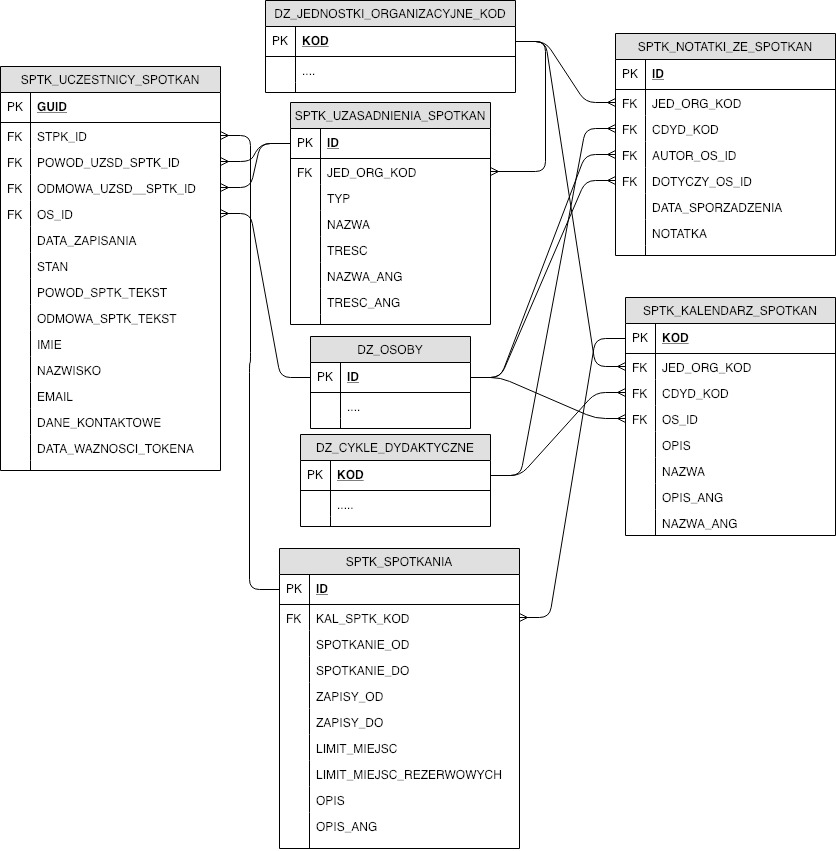
\includegraphics[width=\linewidth]{schemat.jpg}
  \caption{Schemat bazy danych (tylko najważniejsze tabele i pola)}
  \label{fig:schemat}
\end{figure}

%\FloatBarrier
\section{Przykładowe scenariusze użycia modułu}
Dla prostoty przyjęto dzień jako niepodzielną jednostkę czasu.

%\begin{step}
%	\item Lista rezerwowa
	\setlength{\tabcolsep}{8pt}
	
\begin{table}[h]
	\begin{center}
	\centering
	\caption{Lista Rezerwowa}
	\begin{tabularx}{\textwidth}{ v X n }
	\toprule
	Dzień & Student & Spotkanie1 \\
	\midrule
	1  &    & Definicja \\
	\midrule[0.001em]
	2  & Dostępne spotkania: Spotkanie1.\newline Zapisanie na Spotkanie1, miejsce na~liście rezerwowej. & Zapisy \\
	\midrule[0.001em]
	3  & Kilka miejsc w kolejce zostaje zwolnionych, dostaje się na spotkanie  & Akceptacja \\
	\midrule[0.001em]
	4  &   & Spotkanie \\
	\bottomrule
	\end{tabularx}
	\end{center}
\end{table}
	
Poniższe trzy przykłady zakładają istnienie tokenów, które nie zostały zaimplementowane w ramach niniejszej pracy.

%\item Token przeniesienia
\begin{table}[h]
	\begin{center}
	\centering
	\caption{Token przeniesienia}
	\begin{tabularx}{\columnwidth}{ v X n n }
	\toprule
	Dzień & Student & Spotkanie1 & Spotkanie2\\
	\midrule
	1  &    & Definicja & Definicja \\
	\midrule[0.001em]
	2  & Dostępne spotkania: Spotkanie1. \newline Zapisanie na Spotkanie1, miejsce na liście rezerwowej & Zapisy & \\
	\midrule[0.001em]
	3  & Nie dostaje się na spotkanie, pozostaje w rezerwie.  & Akceptacja & \\
	\midrule[0.001em]
	4  & Dostaje token przeniesienia. \newline Dostępne spotkania: Spotkanie2. \newline Przenosi się na Spotkanie2 & Spotkanie & \\
	\midrule[0.001em]
	5  &  &  & Zapisy\\
	\midrule[0.001em]
	6  & Dostaje się na spotkanie &  & Akceptacja\\
	\midrule[0.001em]
	7  &  &  & Spotkanie\\
	\bottomrule
	\end{tabularx}
	\end{center}
\end{table}
	
%\item Token przeniesienia pozwala na przeniesienie tylko do nierozpoczętej rejestracji
\begin{table}[h]
	\begin{center}
	\centering
	\caption{Token przeniesienia pozwala na przeniesienie tylko do spotkania, którego okres zapisów jeszcze sie nie zaczął}
	\begin{tabularx}{\columnwidth}{ v X n n n }
	\toprule
	Dzień & Student & Spotkanie1 & Spotkanie2 & Spotkanie3\\
	\midrule
	1  &    & Definicja & Definicja &\\
	\midrule[0.001em]
	2  & Dostępne spotkania: Spotkanie1. \newline Zapisanie na Spotkanie1, miejsce na liście rezerwowej. & Zapisy &  &\\
	\midrule[0.001em]
	3  & Nie dostaje się na spotkanie, pozostaje w rezerwie.  & Akceptacja &  &\\
	\midrule[0.001em]
	4  & Dostaje token przeniesienia.\newline Dostępne spotkania: brak & Spotkanie & Zapisy &\\
	\midrule[0.001em]
	5  & Token wygasa &  & Zapisy & Definicja\\
	\midrule[0.001em]
	6  &  &  & Akceptacja & Zapisy\\
	\bottomrule
	\end{tabularx}
	\end{center}
\end{table}
	
	\newpage
%\item Wiele tur jednocześnie
\begin{table}[h]
	\begin{center}
	\centering
	\caption{Wiele tur jednocześnie}
	\begin{tabularx}{\columnwidth}{ v X m m }
	\toprule
	Dzień & Student & Spotkanie1 & Spotkanie2 \\
	\midrule
	1  &    & Definicja & Definicja \\
	\midrule[0.001em]
	2  & Dostępne spotkania: Spotkanie1. \newline Zapisanie na Spotkanie1, miejsce na liście rezerwowej. & Zapisy & Zapisy\\
	\midrule[0.001em]
	3  & Nie dostaje się na spotkanie, pozostaje w rezerwie.  & Akceptacja & Zapisy\\
	\midrule[0.001em]
	4  & Dostaje token przeniesienia.\newline Dostępne spotkania do przeniesienia: brak.\newline Dostępne spotkania do zapisu: Spotkanie2.\newline Zapisanie na Spotkanie2 & Spotkanie & Zapisy\\
	\midrule[0.001em]
	5  & Token wygasa &  & Akceptacja \\
	\midrule[0.001em]
	6  &  &  & Spotkanie \\
	\bottomrule
	
	\end{tabularx}
	\end{center}
\end{table}
%\end{step}

\chapter{Implementacja} \label{chap:implementacja}
\section{USOS}
USOS jest skomplikowanym systemem, rozwijanym przez lata. Składa się z wielu komponentów odpowiadających za różne funkcjonalności potrzebne do obsługi studiów. Ze względu na zróżnicowane okresy powstawania oraz przeznaczenie, różnią się między sobą znacząco technologią wykonania, a zasada współdziałania całego systemu jest bardzo skomplikowana.
Składowe, z którymi mieliśmy styczność podczas naszej pracy, to:
\begin{itemize}
\item USOSadm w Javie -- moduł przeznaczony dla pracowników administracji,
\item USOSweb -- moduł przeznaczony dla studentów,
\item baza danych Oracle -- centralna baza danych USOS, posiada bogatą wewnętrzną logikę odpowiadającą między innymi za dostęp do danych, uprawnienia użytkownika są sprawdzane na poziomie bazy danych, bezpośrednio kontaktuje się z nią USOSadm \cite{rfd},
\item baza danych MySQL -- baza danych, z którą łączy się USOSweb, w większości kopia bazy danych Oracle \cite{wikibd},
\item Migrator -- moduł odpowiedzialny za synchronizację baz danych, ponieważ ruch w systemie USOS jest rozproszony pomiędzy wiele aplikacji i baz danych, Migrator dba o zachowanie spójności danych z centralną bazą podstawową (system USOS) a bazami satelitarnymi (bazami aplikacji stowarzyszonych, na przykład USOSweb) wykonując częste, okresowe migracje \cite{wdr}.
\end{itemize}

\section{USOSadm} \label{sec:impusos}

\subsection{Informacje ogólne}
Celem prac w obrębie USOSadm było zaimplementowanie funkcjonalności przy wykorzystaniu przyjętych praktyk programistycznych. Jej zakres obejmował następujące mechanizmy:
\begin{itemize}
\item definiowanie nowych kalendarzy spotkań oraz spotkań z pracownikami uczelni,
\item zapisy i akceptowanie zapisów na spotkania studentów,
\item sporządzanie notatek ze spotkań,
\item definiowanie listy najczęstszych powodów zapisów na spotkania.
\end{itemize}

\subsection{Aplikacja kliencka}
Aplikacja kliencka USOSadm to część aplikacji wykonywana na stanowisku klienta. Składa się m.in. z~kodu HTML i~skryptów JavaScript. Działa w przeglądarce internetowej Mozilla Firefox lub Google Chrome \cite{wdr}.

\subsection{Serwer}
Serwer USOSadm odpowiedzialny jest za~większą część logiki aplikacji. Napisany został w Javie. Do tworzenia interfejsu użytkownika wykorzystuje się JavaServer Faces oraz biblioteki komponentów RichFaces \cite{wikijsf}.

\subsection{Komunikacja z bazą danych}
Komunikacja z~bazą~danych została zrealizowana przy pomocy własnego, bogatego API zrealizowanego przy pomocy technologi Hibernate. Technologia Hibernate pozwala na~odwzorowanie danych z~bazy~danych za~pomocą odpowiednio spreparowanych obiektów w~Javie. Klasy mapuje się na tabele, obiekty na wiersze, atrybuty na dane \cite{hibernate}.

\subsection{JavaBean}
Jest to komponent programowy, który może być wielokrotnie używany. Ma cechy takie, jak:
\begin{itemize}
\item prywatne atrybuty, dostępne przez metody zwane akcesorami,
\item udostępnia na zewnątrz metody (na przykład dla przycisku na ekranie),
\item obsługuje zdarzenia (na przykład wyświetla spotkanie po wybraniu kalendarza) \cite{javabean}.
\end{itemize}
Każdą, utworzoną przez nas, tabelę w USOSadm obsługuje oddzielna klasa zgodna z JavaBean.

\subsection{Klasy implementacji}
Aby zaimplementować formularze, stworzono trzy główne klasy oraz trzy dodatkowe:

\begin{itemize}
\item \textsl{KalendarzeSpotkanBean} -- odpowiada za widok Kalendarze spotkań. Ze względu na bogatą funkcjonalność używa kilku dodatkowych modułów:
\begin{itemize}
\item \textsl{SpotkaniaModule} -- obsługuje formularz Spotkania w kalendarzu, w którym wyświetlają się spotkania, po wybraniu kalendarza.
\item \textsl{UczestnicySpotkanModule} -- obsługuje formularz Uczestnicy spotkania, w którym wyświetlają się uczestnicy spotkania, po wybraniu spotkania.
\item \textsl{NotatkiUczestnikowModule} -- obsługuje formularz, w którym wyświetlają się notatki osoby wybranej na formularzu Uczestnicy spotkania.
\end{itemize}
\item \textsl{NotatkiZeSpotkanBean} -- odpowiada za widok Notatki.
\item \textsl{UzasadnieniaSpotkanBean} -- odpowiada za widok Słownik uzasadnień.
\end{itemize}

\subsection{Pobieranie danych}
Bardzo często obiekty w bazie danych odwołują się do innych obiektów z bazy. Przy pracy z danym obiektem może być konieczne skorzystanie z danych pewnych zależnych obiektów. Z uwagi na to wyróżniamy dwa sposoby pobierania zależnych rekordów.

\begin{itemize}
\item Gorliwe -- zależne rekordy pobierane są od razu. Jest to szybszy sposób na pobranie wszystkich danych, lecz w przypadku, kiedy te dane nie są potrzebne, pobieramy potencjalnie duże ilości zbędnych danych.
\item Leniwe -- zależne rekordy pobierane są dopiero później, na żądanie.
\end{itemize}

Przyjętym standardem w USOSadm jest leniwe pobieranie zależnych rekordów. W przypadku, gdy zależne dane są potrzebne (na przykład trzeba je wyświetlić w tabeli), inicjuje się je podczas pobierania danych w klasie \textsl{Service}.

\subsection{Szablony}
Wizualna prezentacja widoków jest definiowana w szablonach. Zgodnie z istniejącymi standardami, każda tabela i formularz posiada swój własny, odrębny szablon.

\subsection{Moduł Spotkania}
Dostęp do modułu Spotkania został umieszczony w menu Studenci, co widać na ekranie~\ref{fig:modspoadm}.

\subsection{Kalendarze spotkań}
Widok Kalendarze spotkań ma rozbudowaną strukturę. Widać to na ekranie \ref{fig:kalenadm}. Należy wybrać kalendarz w górnej części ekranu. Wtedy na 
formularzu Spotkania w kalendarzu będą widoczne spotkania z tego kalendarza. Po wybraniu spotkania, na formularzu Uczestnicy spotkania, pojawią się 
uczestnicy tego spotkania. Po wybraniu uczestnika na dole ekranu można zobaczyć zakładki z szczegółowymi informacjami o powodach jego zapisu oraz 
ewentualnego odrzucenia, oraz jego notatkami ze spotkań. Fragment dolnego formularza, na którym widać notatki studenta jest na ekranie 
\ref{fig:kalennotadm}.

\begin{figure}[!]
  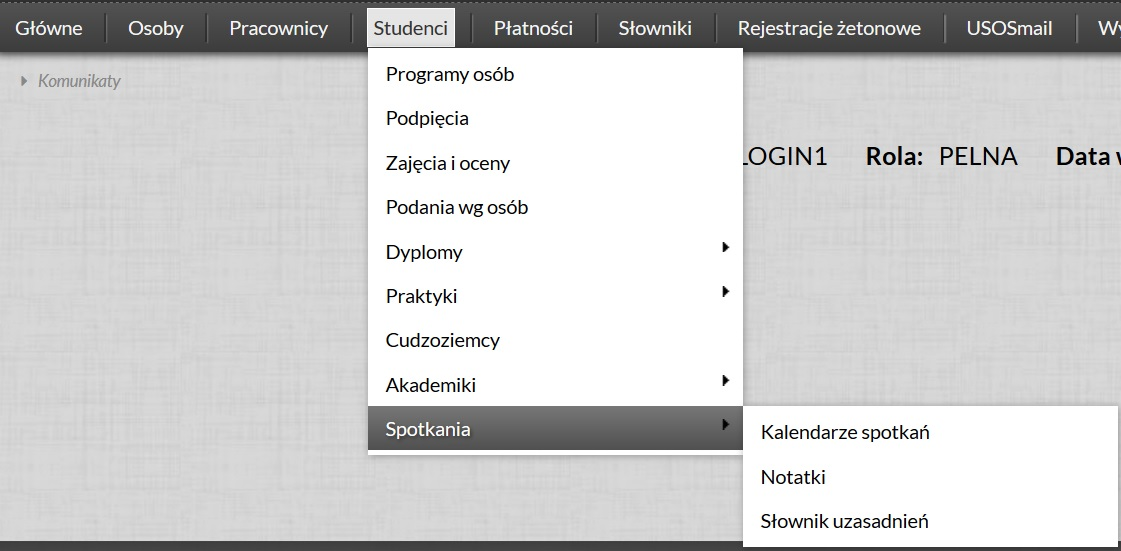
\includegraphics[width=\linewidth]{spotkaniaadm.jpg}
  \caption{Dostęp do modułu Spotkania}
  \label{fig:modspoadm}
\end{figure}

Widok zawiera komplet formularzy do tworzenia i edycji wpisów w modelach. Obejmuje to formularz kalendarzy spotkań, widoczny na ekranie 
\ref{fig:kalenformkalenadm}, formularz spotkań, widoczny na ekranie \ref{fig:kalenformspotkadm}, formularz uczestników spotkania w wersji dla uczestnika 
z systemu USOSadm \ref{fig:kalenformuczusosadm}, oraz spoza systemu \ref{fig:kalenformucznieusosadm}. Formularze te otwiera się odpowiednimi przyciskami 
\textsf{+Dodaj}, które są w lewych górnych rogach odpowiednich formularzy lub przyciskami do edytowania, które są w każdym wierszu z tabeli po prawej 
stronie.

\begin{figure}[!]
  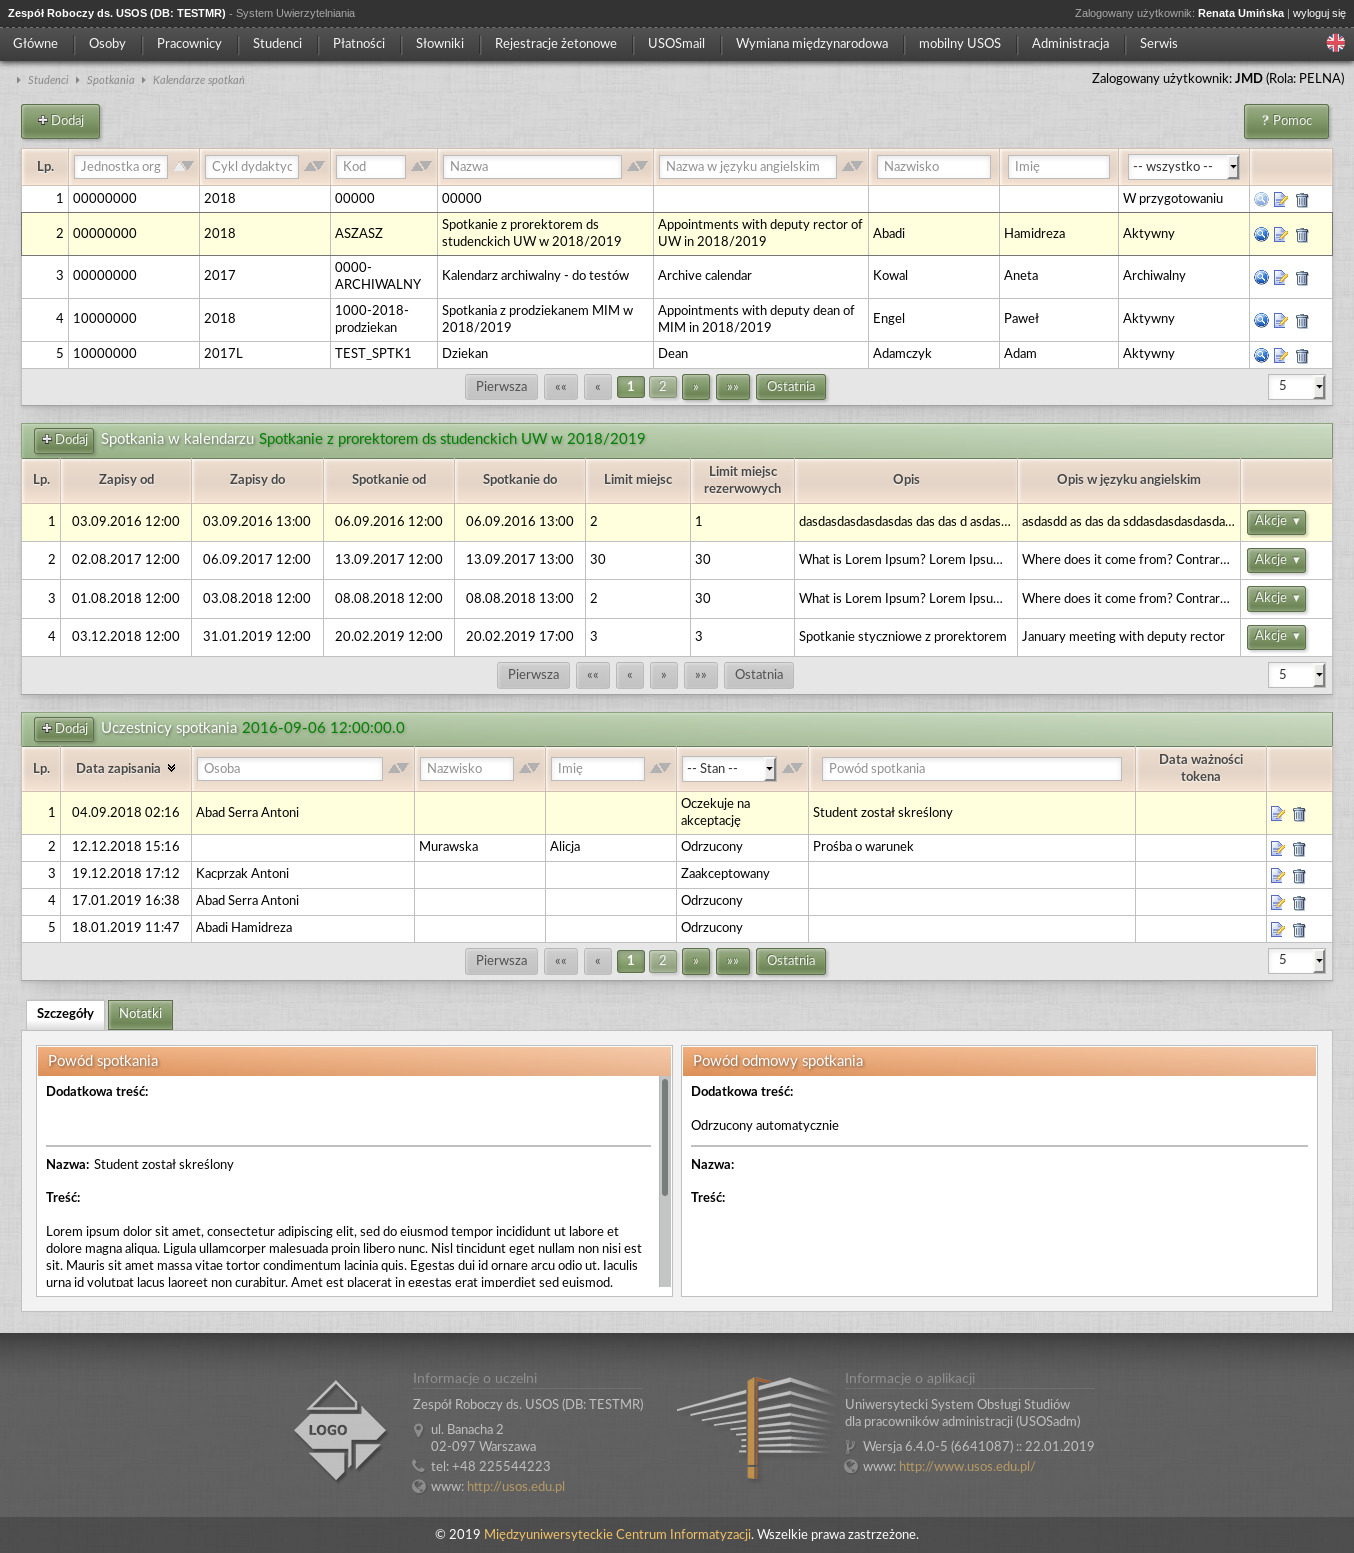
\includegraphics[width=\linewidth]{widok_kalendarzy.jpg}
  \caption{Widok kalendarzy spotkań}
  \label{fig:kalenadm}
\end{figure}

\begin{figure}[!]
  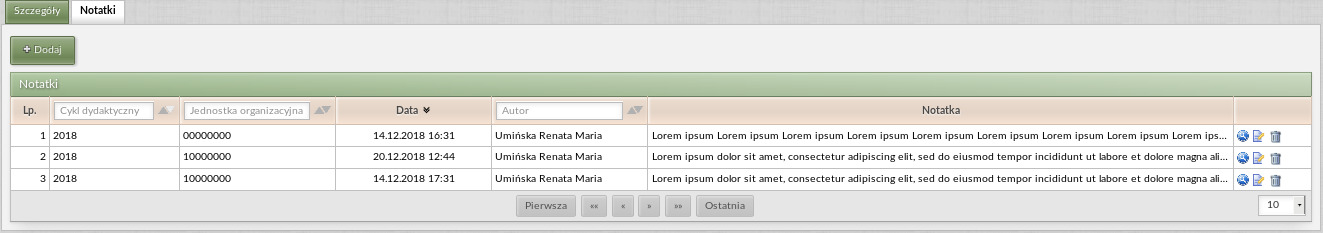
\includegraphics[width=\linewidth]{widok_kalendarzy_tabela_notatek.jpg}
  \caption{Zakładka notatek}
  \label{fig:kalennotadm}
\end{figure}

\begin{figure}[!]
  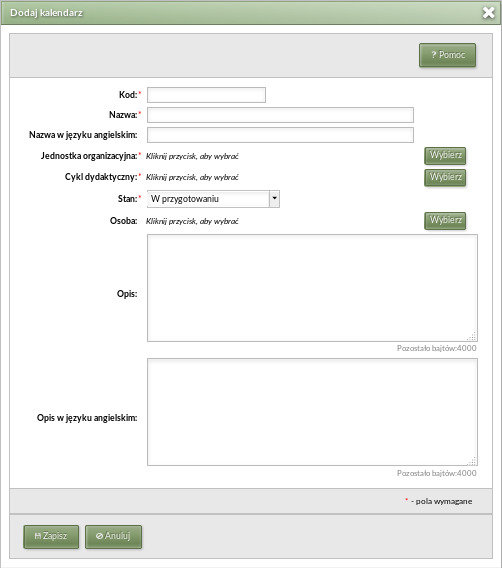
\includegraphics[width=\linewidth]{formularz_kalendarzy.jpg}
  \caption{Formularz dodawania kalendarza spotkań}
  \label{fig:kalenformkalenadm}
\end{figure}

\begin{figure}[!]
  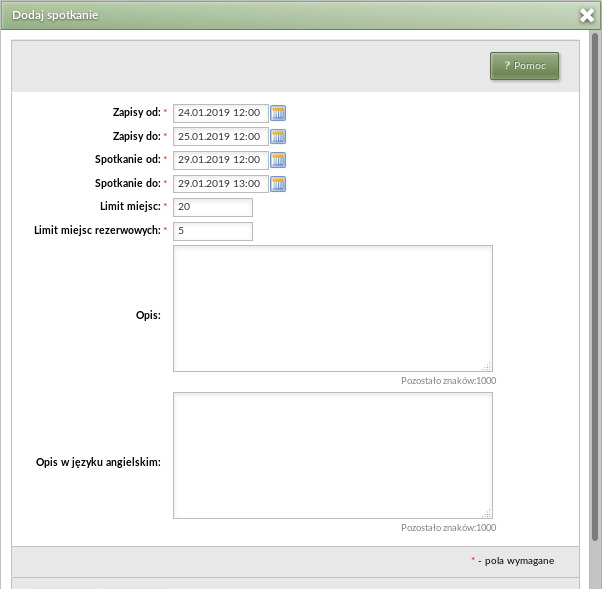
\includegraphics[width=\linewidth]{formularz_spotkan.jpg}
  \caption{Formularz dodawania spotkania}
  \label{fig:kalenformspotkadm}
\end{figure}

\begin{figure}[!]
  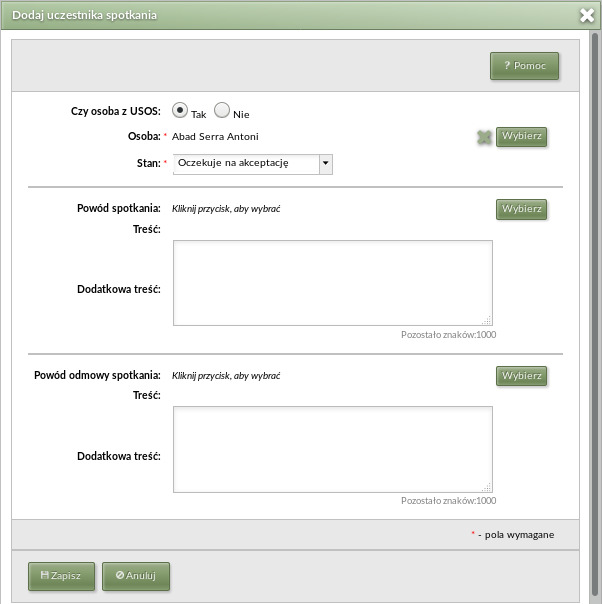
\includegraphics[width=\linewidth]{formularz_uczestnikow_USOS.jpg}
  \caption{Formularz dodawania uczestnika spotkania z USOS}
  \label{fig:kalenformuczusosadm}
\end{figure}

\begin{figure}[!]
  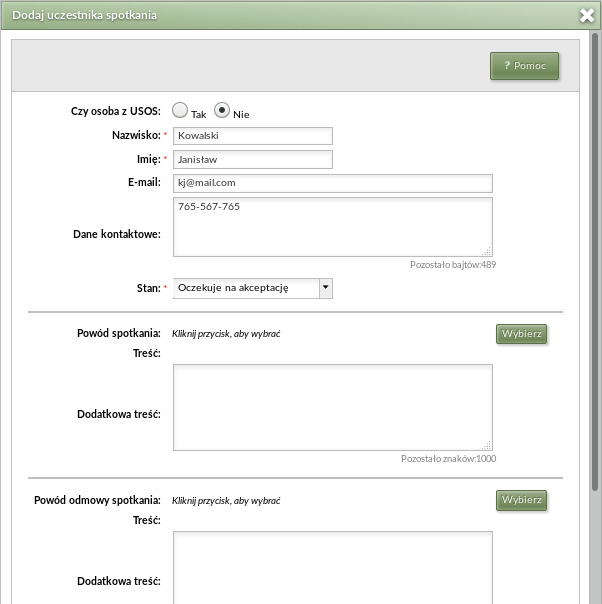
\includegraphics[width=\linewidth]{formularz_uczestnikow_nieUSOS.jpg}
  \caption{Formularz dodawania uczestnika spotkania spoza USOS}
  \label{fig:kalenformucznieusosadm}
\end{figure}

\subsection{Notatki}
Formularz Notatki ma prostą strukturę. Widać to na ekranie \ref{fig:notatki}. Należy wybrać studenta w górnej części ekranu, następnie notatkę w dolnej części ekranu.

Na ekranie \ref{fig:formularz_notatek} widać formularz służący do dodawania lub modyfikowania notatek ze spotkań. Aby otworzyć ten 
formularz należy użyć przycisku \textsf{+Dodaj} po lewej stronie pomiędzy formulrzem, w którym wyświetlają się studenci, a formularzem, w którym są 
notatki lub użyć przycisku do modyfikowania, takie przyciski są po prawej stronie wiersza z tabeli.

\begin{figure}[!]
  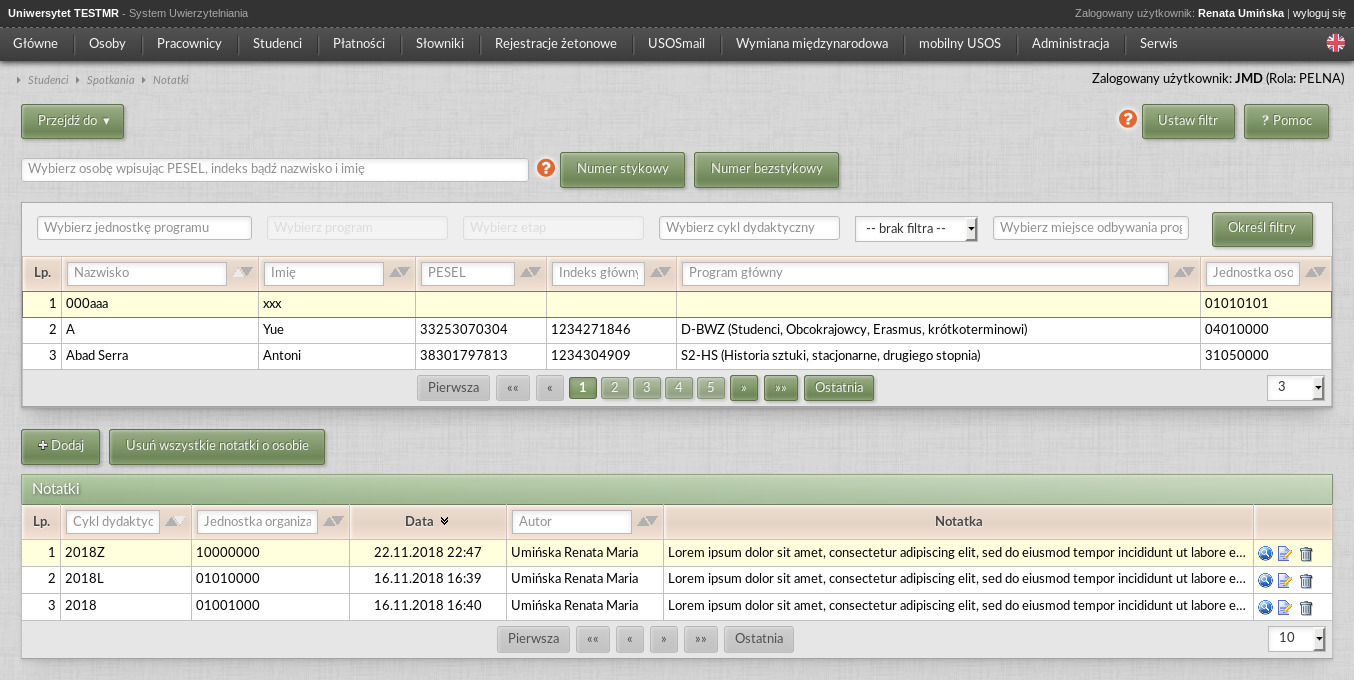
\includegraphics[width=\linewidth]{widok_notatek.jpg}
  \caption{Widok notatek ze spotkań}
  \label{fig:notatki}
\end{figure}

\begin{figure}[!]
  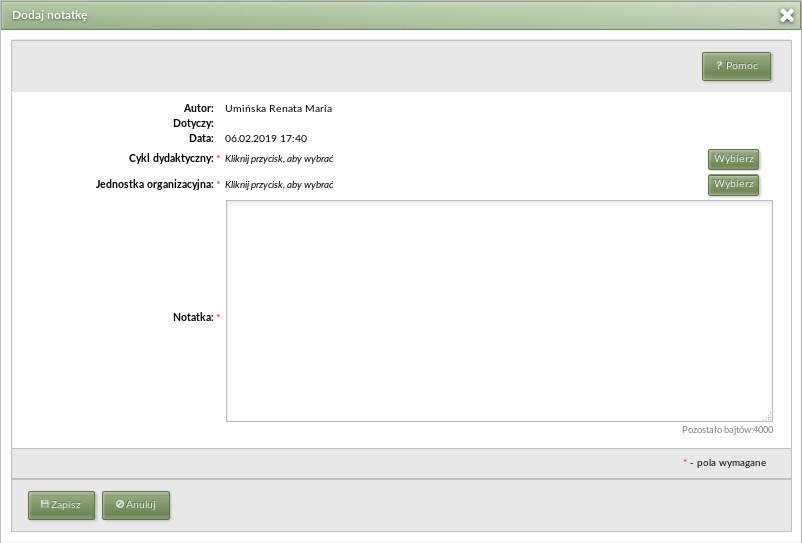
\includegraphics[width=\linewidth]{formularz_notatek.jpg}
  \caption{Formularz dodawania notatki ze spotkania}
  \label{fig:formularz_notatek}
\end{figure}

\subsection{Słownik uzasadnień}
Widok Słownika uzasadnień jest bardzo prosty w budowie i obsłudze. Na ekranie \ref{fig:uzasadnienia} umieszczono: jednostki, typy uzasadnień oraz ich nazwy po polsku i angielsku. Po wybraniu uzasadnienia na dole ekranu pojawi się jego treść po polsku i angielsku.

Po wciśnięciu przycisku \textsf{Dodaj}, przycisku po prawej stronie wiersza z tabeli lub przycisku na dole po lewej stronie pojawi się formularz 
widoczny na ekranie \ref{fig:formularz_uzasadnienia}. Ten formularz służy do dodawania lub modyfikowania uzasadnień.

\begin{figure}[!]
  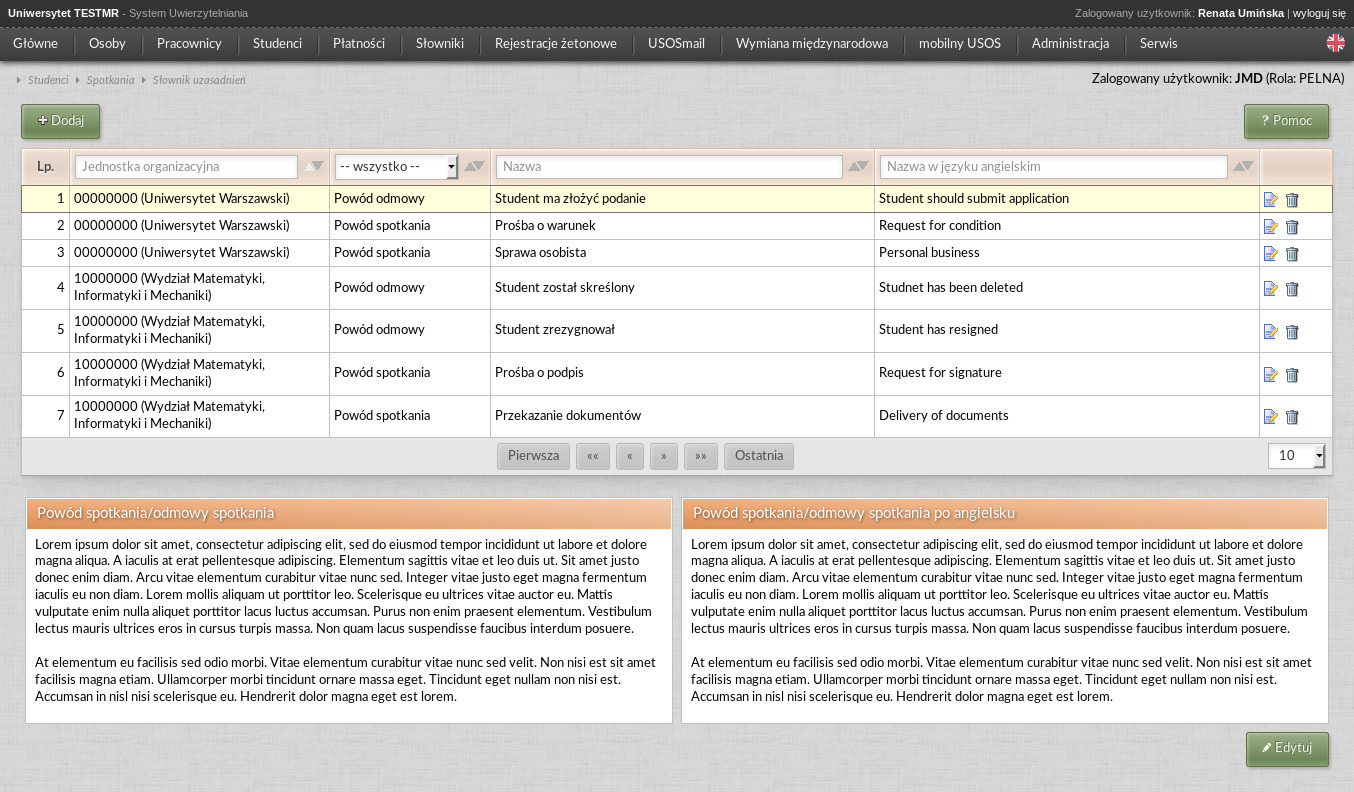
\includegraphics[width=\linewidth]{widok_uzasadnien.jpg}
  \caption{Widok Słownika uzasadnień zapisów na spotkanie}
  \label{fig:uzasadnienia}
\end{figure}

\begin{figure}[!]
  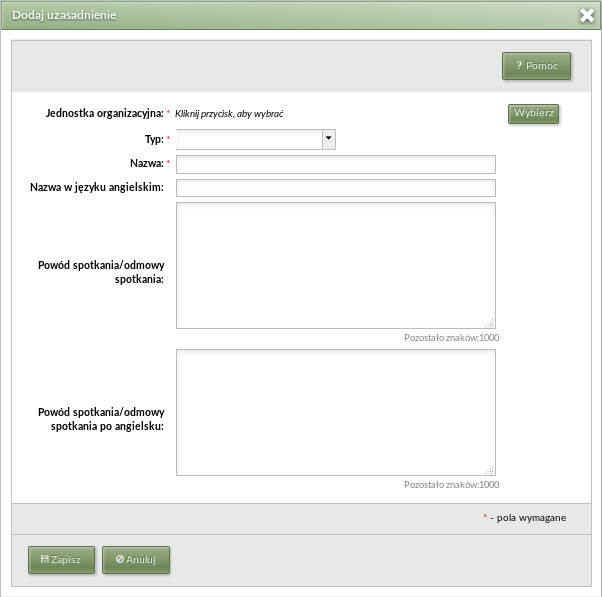
\includegraphics[width=\linewidth]{formularz_uzasadnien.jpg}
  \caption{Formularz dodawania uzasadnienia zapisu na spotkanie}
  \label{fig:formularz_uzasadnienia}
\end{figure}

%subsection{Tokeny}
%Niestety nie udało się zaimplementować mechanizmu tokenów w ramach tego modułu. Pozostaje on jako %możliwa ścieżka dalszego rozwoju funkcjonalności.

%\FloatBarrier
\section{USOSweb} \label{sec:impusosweb}

\subsection{Informacje ogólne}
Implementacja funkcjonalności w USOSweb polegała na jego rozbudowaniu przy pomocy najlepszych w danej chwili praktyk programowania przyjętych przez zespół tworzący i wspierający system USOSweb. Zachowując spójność z pozostałymi częściami systemu, stworzyliśmy moduł pozwalający studentowi na:
\begin{itemize}
  \item{wyświetlanie informacji o jednostkach oferujących spotkania,}
  \item{wybór jednostki, w ramach której odbywa się interesujące studenta spotkanie,}
  \item{wyświetlanie kalendarza spotkań wybranej osoby lub jednostki,}
  \item{wyświetlanie terminów spotkań dla każdego kalendarza wraz ze wszystkimi niezbędnymi informacjami (zajętość miejsc, stan zapisów...),}
  \item{wykonywanie dostępnych akcji związanych ze spotkaniem:
  \begin{itemize}
    \item{wpisywanie się na listę główną lub rezerwową,}
    \item{wypisywanie się,}
    \item{podgląd aktualnego stanu zapisu na spotkanie, w tym informacje takie, jak liczba dostępnych miejsc.}
  \end{itemize}
}
\item{wyświetlanie spotkań związanych ze studentem (czyli takich, na które student jest albo był zapisany).}
\end{itemize}

Dużą uwagę zwróciliśmy na kontrolę dostępu. Pozwalamy studentowi wykonywać tylko te akcje z danymi (na przykład zapisami na spotkania), do których w danej chwili ma on dostęp. W tym celu przy każdym zapytaniu do serwera, wysyłanym z aplikacji klienckiej albo przeglądarki, sprawdzamy, czy użytkownik jest zalogowany oraz czy ma dostęp do danej akcji. Nie zapomnieliśmy również o bezpieczeństwie. Moduł posiada zabezpieczenie przeciwko potencjalnym atakom, więcej na ten temat można przeczytać w sekcji \ref{subsec:bezpiecz}. Staraliśmy maksymalizować użycie gotowych modułów, stworzonych w USOSwebie, minimalizując tym samym duplikowanie kodu.

\subsection{Opis działania systemu USOSweb}
Jak każda aplikacja webowa, system USOSweb składa się z niżej opisanych elementów.
\begin{itemize}
  \item
  Część serwerowa -- program działający na zdalnym komputerze podłączonym do sieci Internet (w USOSweb jest zaimplementowany w PHP).
  \item
  Aplikacja kliencka -- program, działający na komputerze użytkownika, łączący się z aplikacją serwerową (zaimplementowany w JS).
\end{itemize}


Do zrozumienia dalszego opisu implementacji części systemu USOSweb niezbędne są następujące definicje.
\begin{itemize}
  \item
  Akcja -- klasa obiektów, reprezentujących interakcje części klienckiej i serwerowej. Każde zapytanie do serwera (GET, POST, ...) powinno mieć zdefiniowaną akcję, która opisuje zachowanie serwera dla danego zapytania. W sensie programistycznym każda osobna akcja jest klasą (w języku PHP), która naśladuje klasę Action.
  \item
  Użytkownik -- student albo pracownik, mający konto w systemie CAS, korzystający z systemu USOSweb.
  \item
  Zalogowany użytkownik -- użytkownik, który wykonał procedurę logowania się. Kontekst zalogowanego użytkownika zawiera identyfikator, imię i nazwisko oraz wiele innych pomocniczych informacji. 
\end{itemize}

Aplikacja serwerowa oparta jest na kontrolerze, zaimplementowanym w języku PHP, który dostaje w parametrach GET opis akcji, jaką użytkownik chcę wykonać. Każda akcja zaimplementowana jest jako osobna klasa języka PHP (akcja obsługuje całą logikę, ona tworzy wynikowe dane i ewentualnie powoduje efekty uboczne). Za pomocą plików konfiguracyjnych (actions.xml) akcje wiążą się z szablonami (szablony odpowiadają za format wyświetlania danych, które są wynikiem akcji). Akcję mogą, a czasami muszą, korzystać z dodatkowych modułów, które tworzymy jako osobne statyczne albo niestatyczne klasy. Każdy moduł ma zestaw swoich akcji. Poza tym aplikacja serwerowa posiada statyczne klasy, znajdujące się w folderze Utils, będące zbiorem pomocniczych narzędzi (na przykład funkcji albo stałych).

\subsection{Akcje}
Podczas implementacji modułu spotkań, powstało pięć akcji.
\begin{itemize}
\item{\textsl{MojeSpotkaniaAction}}

Akcja odpowiada za wyświetlanie spotkań związanych z zalogowanym studentem.
\item{\textsl{SpotkaniaJednostkiAction}}

Akcja odpowiada za wyświetlanie kalendarzy spotkań wraz z terminami tych spotkań oraz związanych z nimi informacji w wybranej jednostce.
\item{\textsl{WyborJednostkiAction}}

Akcja odpowiada za wyświetlanie jednostek i informacji o liczbie spotkań w każdej z jednostek. Przyjmuje dodatkowy parametr w GET, który włącza lub ~wyłącza ograniczenie listy jednostek tylko do tych, które są związane ze~studentem.
\item{\textsl{ZapisNaSpotkanieAction}}

Akcja odpowiada za tworzenie formularza, pozwalającego na wykonywanie przez studenta dostępnych działań z~danym~spotkaniem. Akcja przyjmuje w GET informację o~spotkaniu, czyli identyfikator spotkania z bazy i tworzy odpowiedni formularz dla studenta w~zależności od tego, co zalogowany student może zrobić ze~wskazanym~spotkaniem w~danym~momencie.
\item{\textsl{ZmianaZapisuNaSpotkanieAction}}

Akcja odpowiada za~zmianę stanu zapisu zalogowanego studenta na dane spotkanie. Jest to jedyna akcja w~danym module, która zmienia dane w~bazie danych. Przyjmuje ona parametry zapytania w postaci POST i~sprawdza CSRF token w celu zabezpieczenia się przed atakami CSRF. Dla każdego zapytania przed modyfikowaniem danych w bazie na początku jest prowadzony proces tak zwanej walidacji w~celu uniemożliwienia wykonania niepoprawnych zmian.
\end{itemize}
\subsection{Szablony}
USOSweb korzysta z szablonów Smarty, które są powiązane z~akcjami za~pomocą plików konfiguracyjnych i~zapewniają odpowiednią prezentację danych powstających w~wyniku danej akcji. W~module~spotkań utworzyliśmy pięć szablonów.
\begin{itemize}
\item{\textsl{FormularzSpotkania}}

Formularz, który wyświetla się w~oknie~modalnym i pozwala na wykonanie przez studenta dozwolonej akcji związanej ze spotkaniem.
\item{\textsl{SpotkaniaJednostki}}

Rozwijana lista cykli, gdzie domyślnie rozwinięte są tylko aktywne cykle. Każdy cykl zawiera listę kalendarzy spotkań. Dla każdego kalendarza wyświetlany zostaje opis osoby prowadzącej spotkania i nazwa kalendarza spotkań. Zawiera on również listę dostępnych terminów i~przycisk pozwalający na pokazanie także niedostępnych terminów.
\item{\textsl{MojeSpotkania}}

Lista spotkań związanych ze studentem. Widok jest identyczny z~widokiem spotkań jednostki, ale pokazywane są tylko spotkania i~kalendarze związane z danym studentem, czyli takie spotkania, na które jest on zapisany. Nie ma żadnych ograniczeń na jednostkę, w której dane spotkanie się odbywa.
\item{\textsl{Spotkanie}}

Szablon pomocniczy używany w szablonie \textsl{FormularzSpotkania}.
\item{\textsl{WyborJednostki}}

Lista jednostek z informacją o liczbie kalendarzy spotkań w danej jednostce.
\end{itemize}
\subsection{Moduły pomocnicze}
Często akcje w USOSweb wykonują te same czynności, jak na przykład pobranie kontekstu zalogowanego użytkownika lub nazwy jednostki na podstawie kodu albo utworzenie struktury pozwalającej na wyświetlanie tabeli z~danymi na~podstawie zapytania.
W naszym rozwiązaniu zostały utworzone cztery moduły pomocnicze.
\begin{itemize}
\item{\textsl{CyklDydaktyczny}}

Klasa jest modelem cyklu dydaktycznego. Zawiera jedną statyczną metodę pozwalającą na pobranie z~bazy danych informacji o~wszystkich kalendarzach spotkań w cyklu dla danej jednostki wraz z terminami spotkań i~kontekstem każdego osobnego spotkania dla~użytkownika. Funkcja ta wykonuje stałą~liczbę zapytań do~bazy~danych.
\item{\textsl{KalendarzSpotkan}}

Klasa jest modelem kalendarza spotkań i~posiada metodę statyczną, pozwalającą na~pobranie z~bazy~danych informacji o~wszystkich kalendarzach spotkań i~spotkaniach dla każdego z~kalendarzy. Wykonuje 2 zapytania do bazy danych.
\item{\textsl{SpotkanieOsoba}}

Klasa jest modelem opisującym stan spotkania w~kontekście danej osoby. Ma dużą liczbę niestatycznych funkcji pomocniczych, wykorzystywanych w wielu miejscach modułu spotkań.
\item{\textsl{SpotkaniaUtils}}

Zestaw funkcji pomocniczych.
\end{itemize}

\subsection{Wybór jednostki}
Na ekranie \ref{fig:wszjweb} jest widoczna lista wyboru spośród wszystkich dostępnych jednostek (a nie tylko jednostek związanych ze studentem) oferujących spotkania. Jeśli jest tylko jedna, to użytkownik zostanie przeniesiony do kalendarzy tej jednostki. 

Podobnie wygląda ekran \enquote{Moje jednostki}. Na tym ekranie są tylko jednostki studenta. Jeśli jest tylko jedna, to użytkownik zostanie przeniesiony do kalendarzy tej jednostki.

\subsection{Wybór spotkania}

Na ekranie \ref{fig:kalweb} są widoczne dwa kalendarze spotkań. Aby zapisać się, należy kliknąć odpowiedni przycisk.

Na ekranie \ref{fig:zapisweb} student, który chce zapisać się powinien wybrać powód zapisu z listy, ewentualnie wpisać komentarz tekstowy i kliknąć przycisk \textsf{ZAPISZ}.

\subsection{Moje spotkania}

Na ekranie \ref{fig:mojeweb} widać spotkania, na które student złożył prośbę o zapisanie. Można sprawdzić, czy prośba została zaakceptowana.

%\FloatBarrier

\begin{figure}[!]
  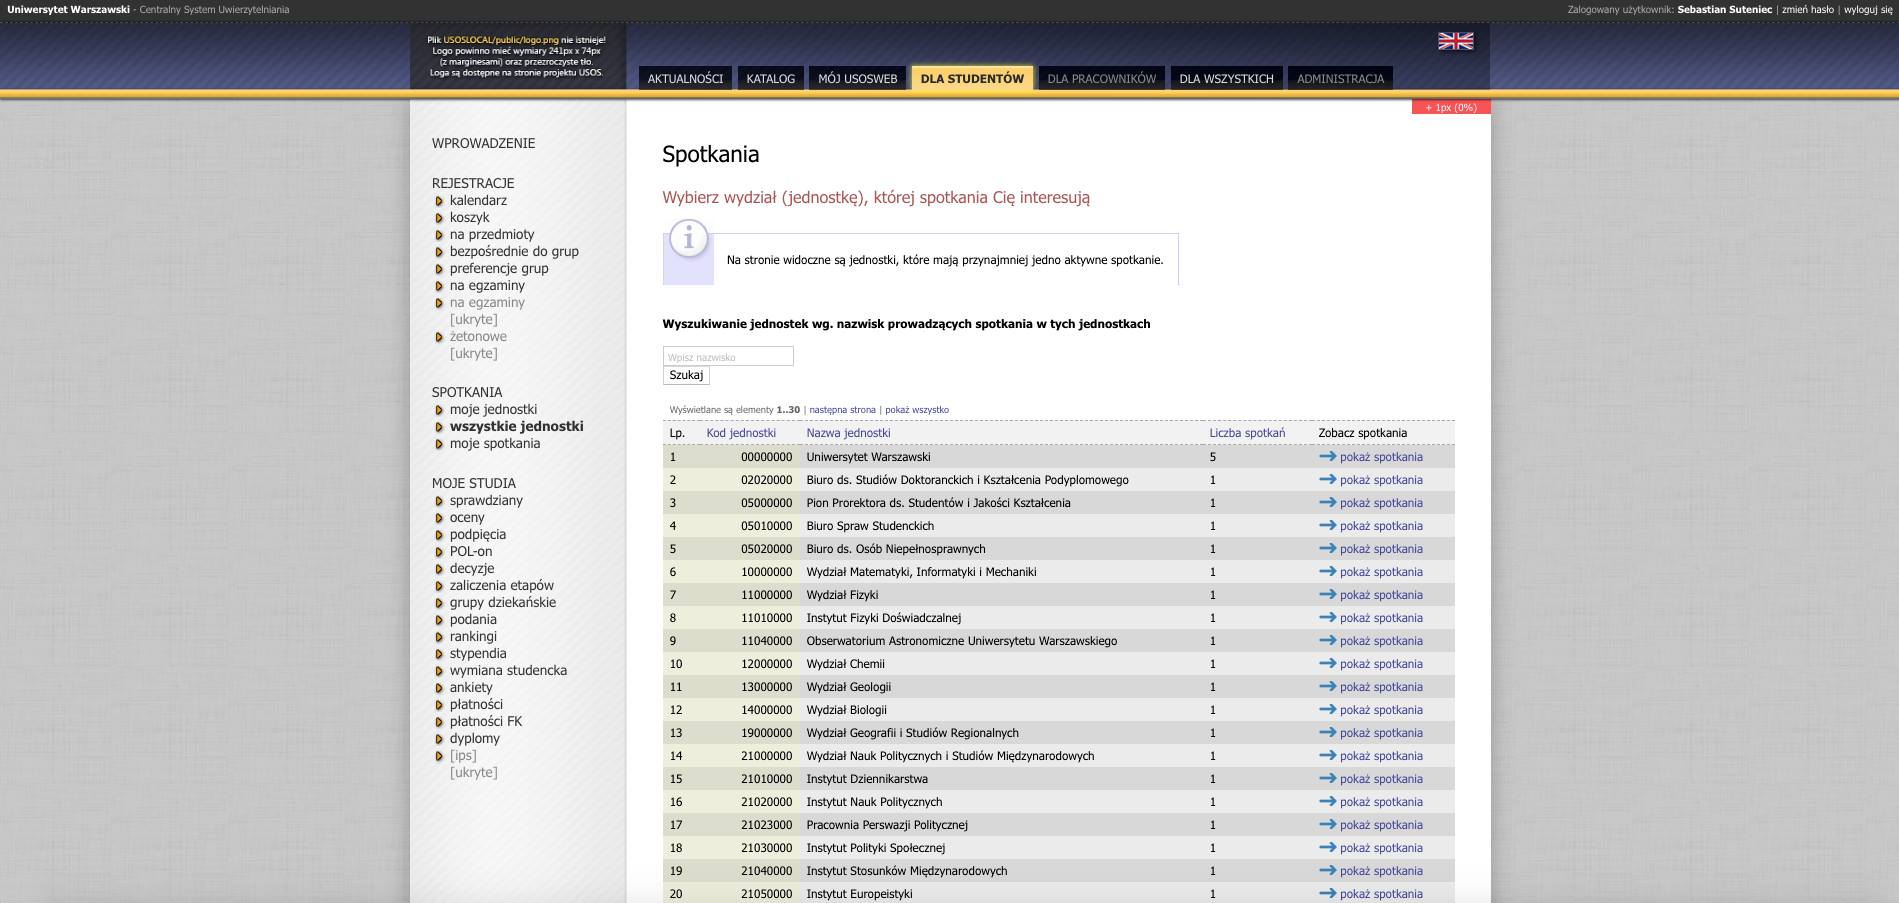
\includegraphics[width=\linewidth]{wszystkie_jednostki_usosweb.jpg}
  \caption{Wszystkie jednostki}
  \label{fig:wszjweb}
\end{figure}

\begin{figure}[!]
  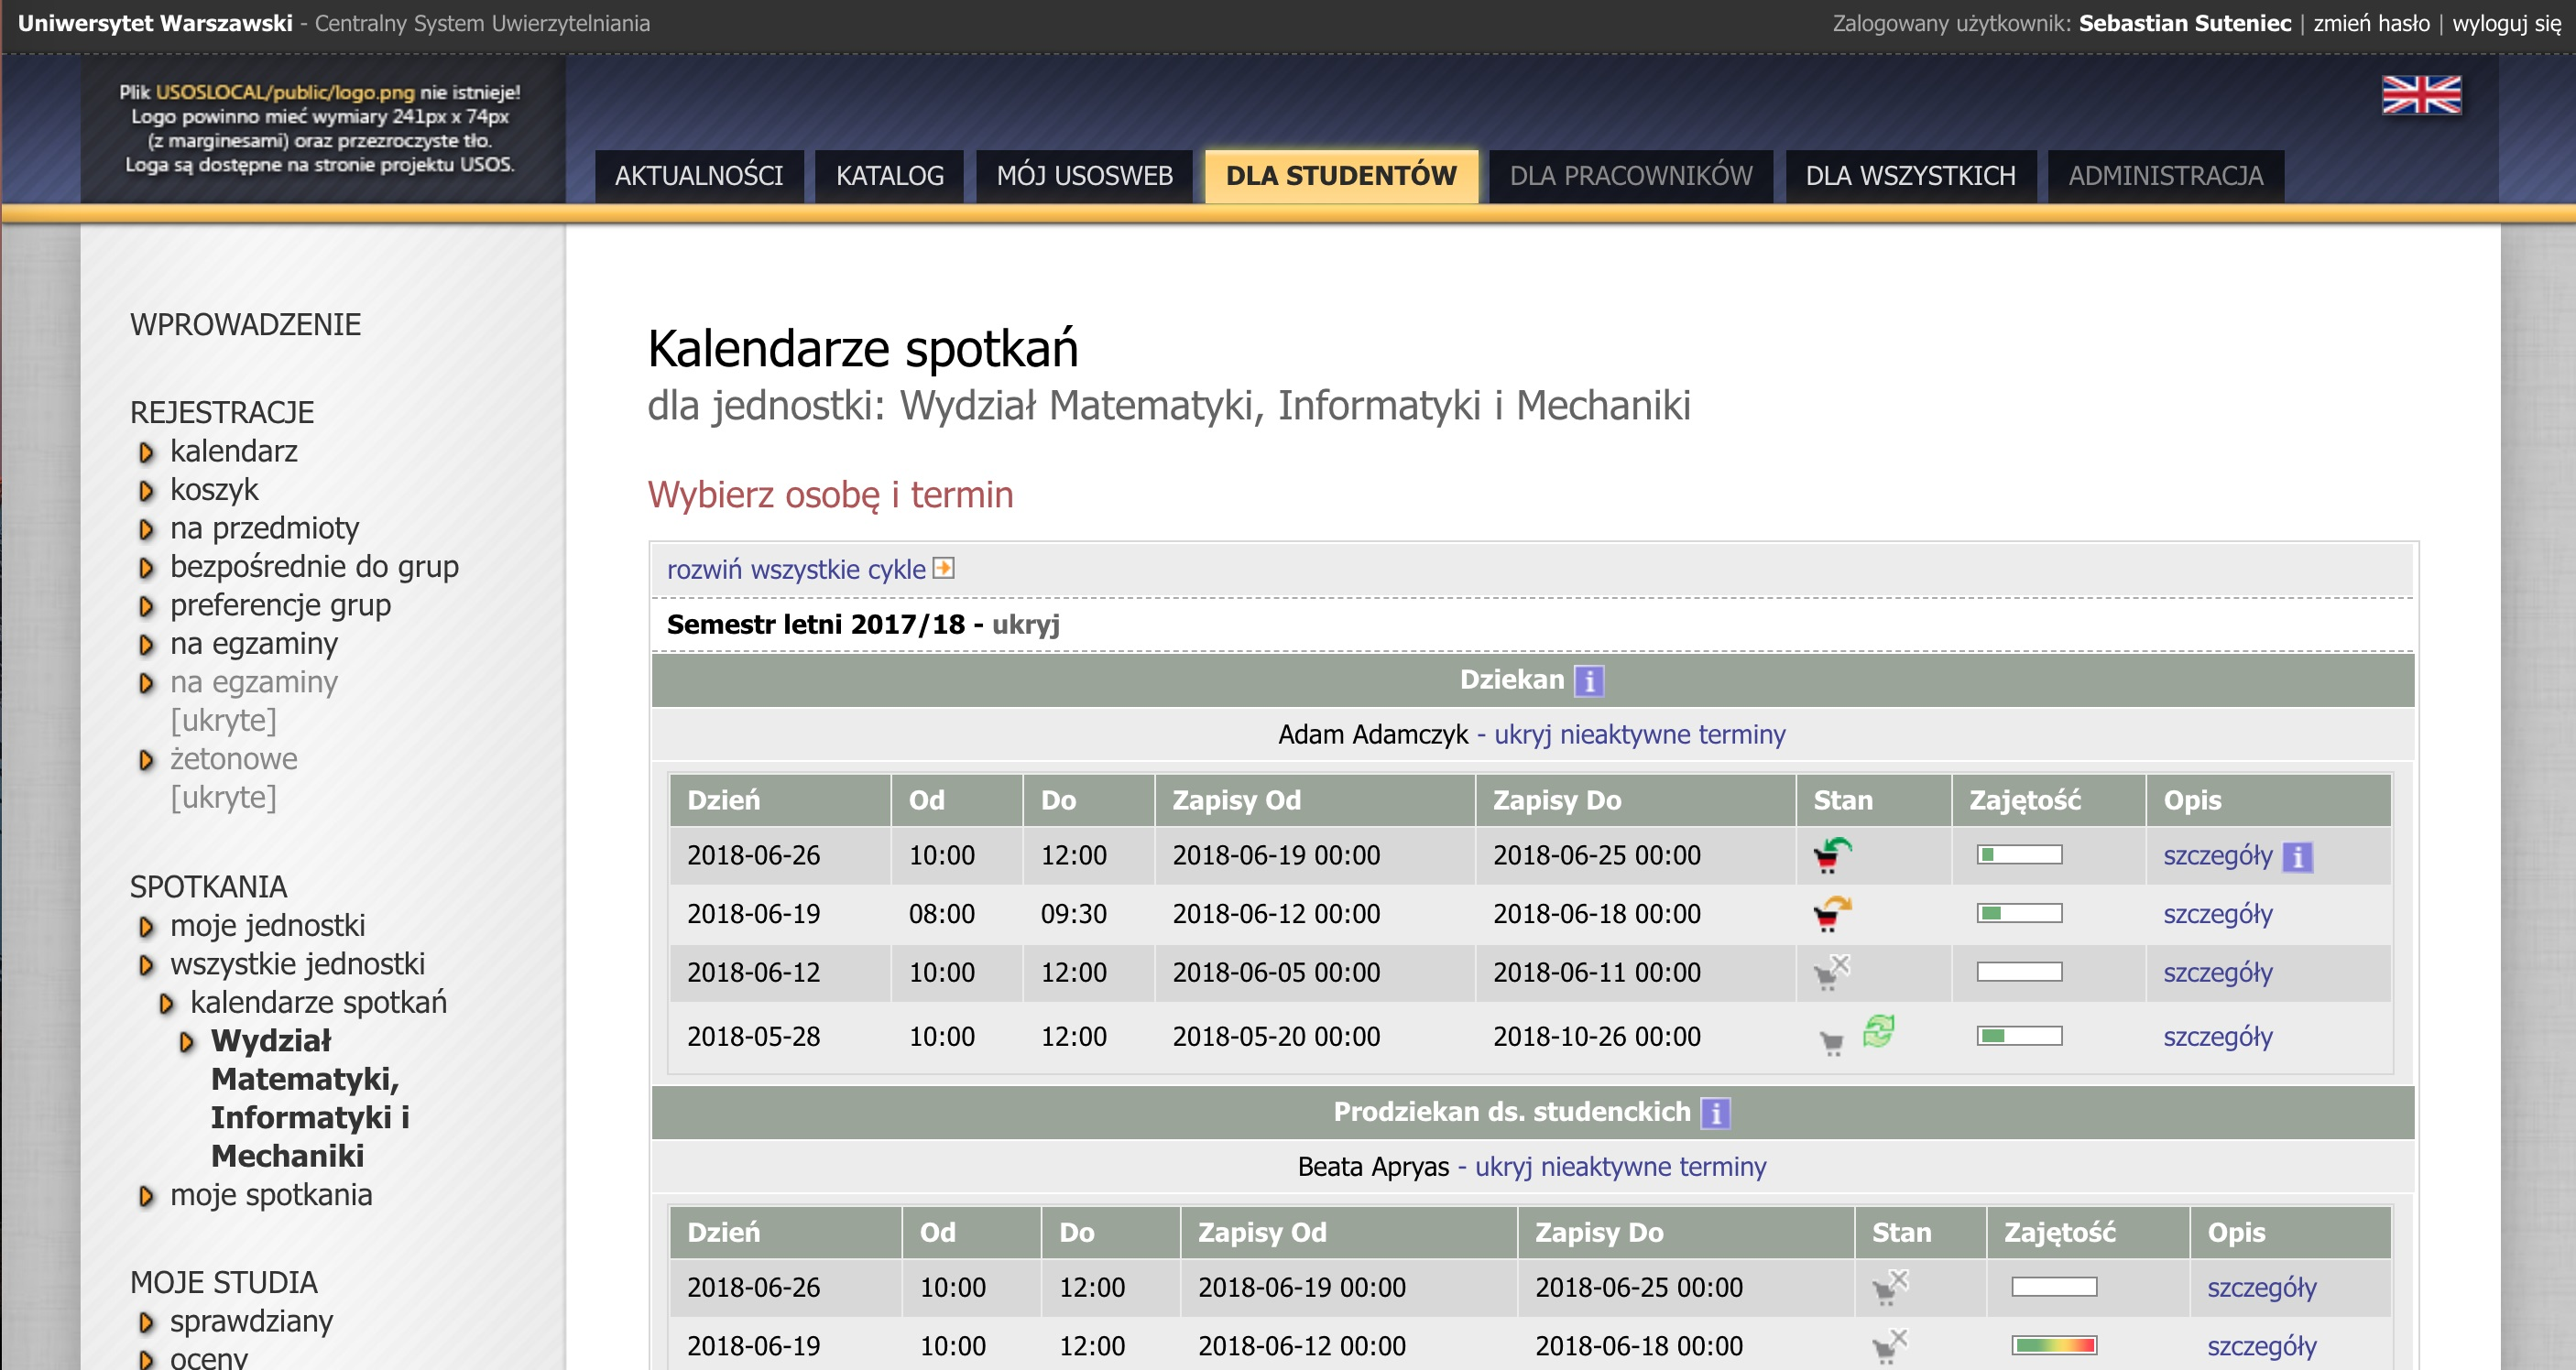
\includegraphics[width=\linewidth]{kalendarzUSOSweb.jpg}
  \caption{Kalendarze spotkań}
  \label{fig:kalweb}
\end{figure}

\begin{figure}[!]
  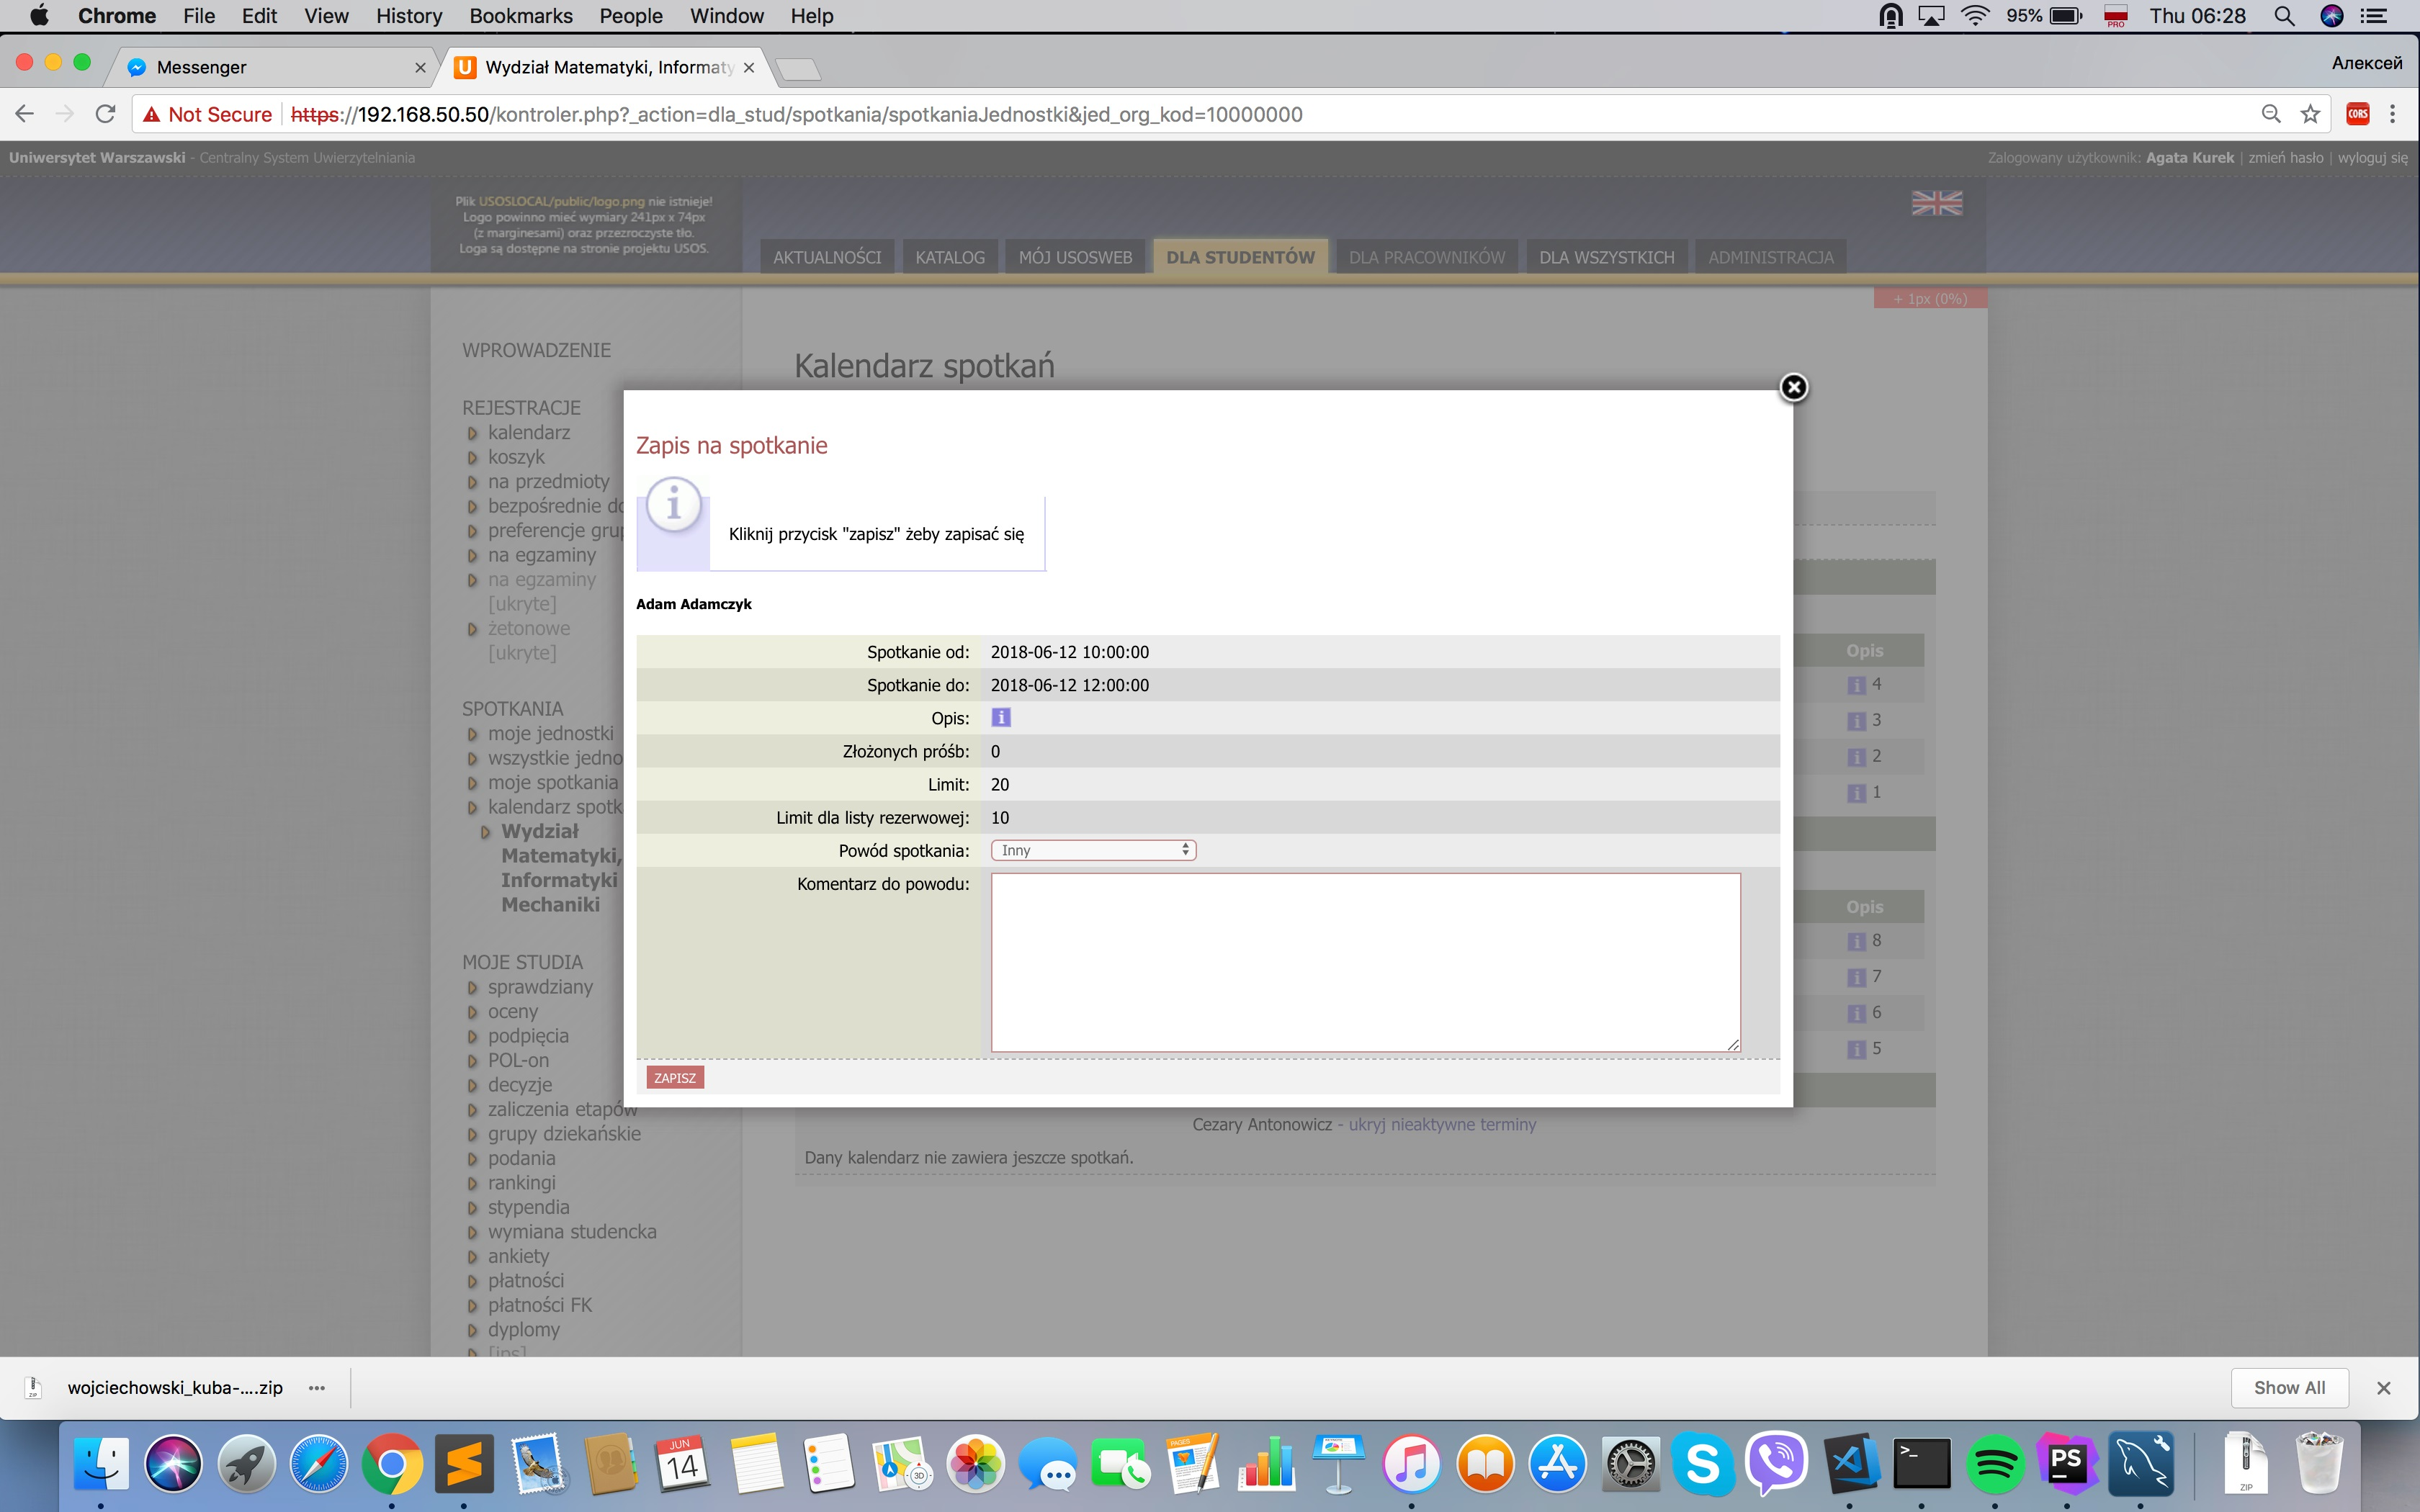
\includegraphics[width=\linewidth]{zapisUSOSweb.jpg}
  \caption{Zapis na spotkanie}
  \label{fig:zapisweb}
\end{figure}

\begin{figure}[!]
  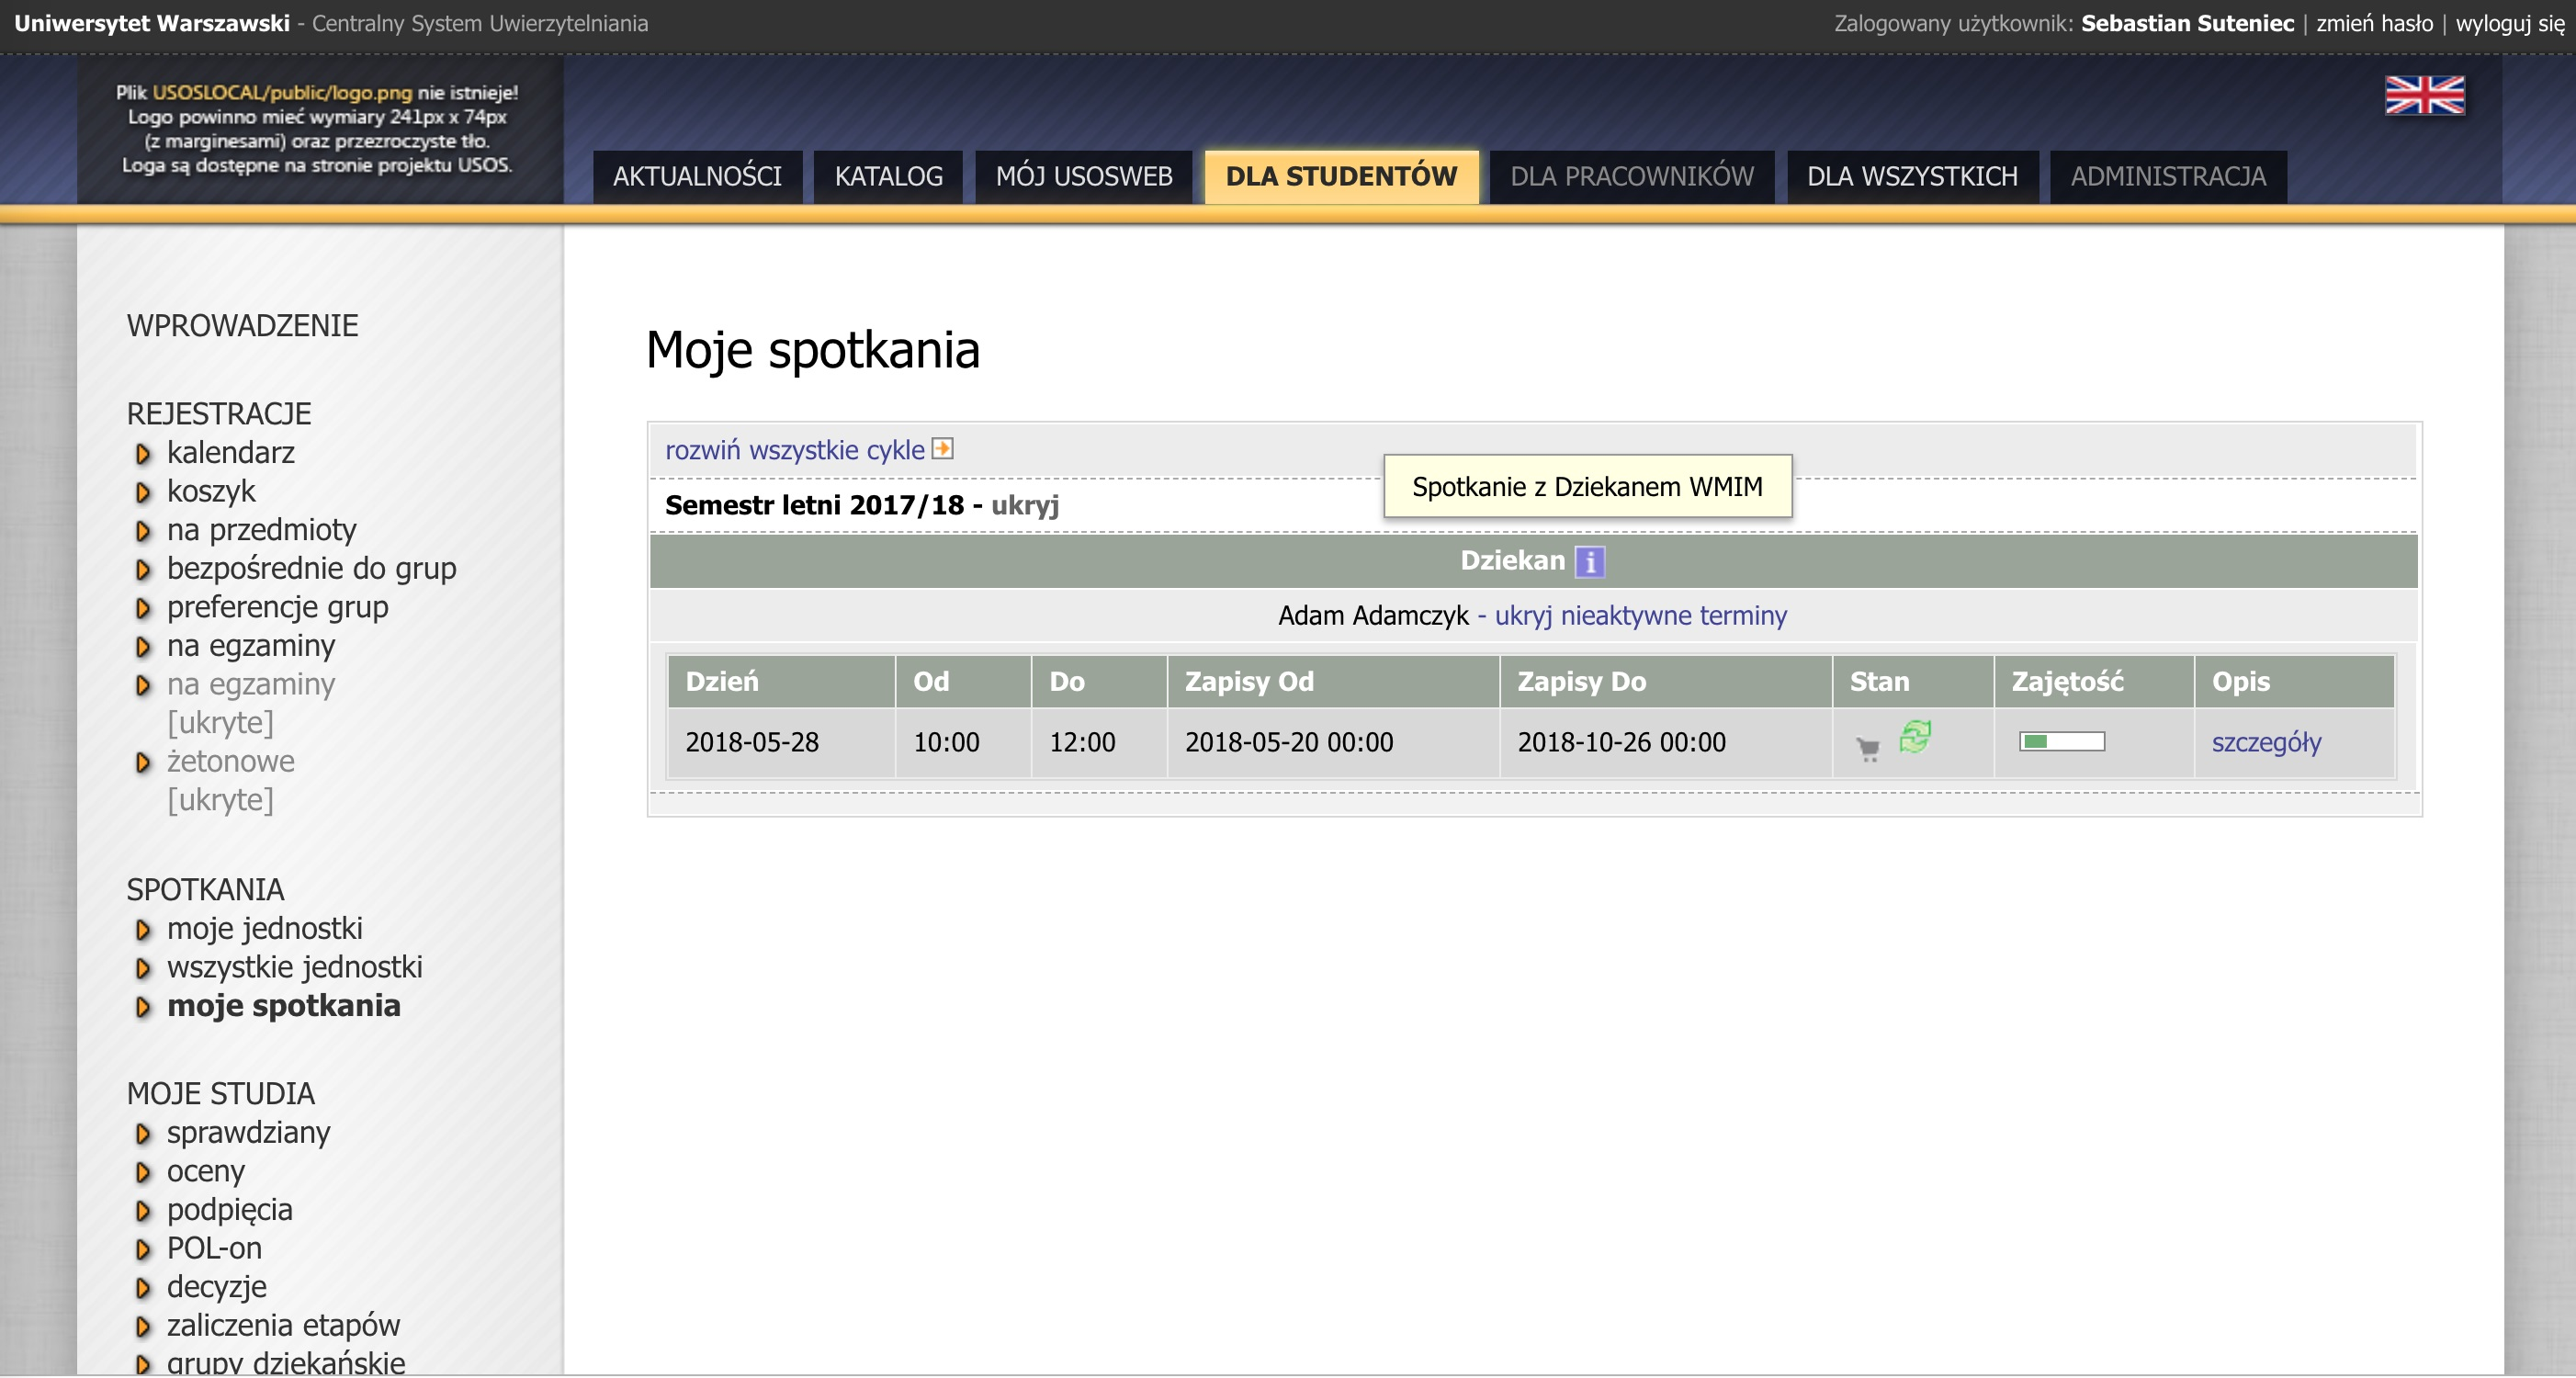
\includegraphics[width=\linewidth]{mojeSpotkaniaUSOSweb.jpg}
  \caption{Moje spotkania}
  \label{fig:mojeweb}
\end{figure}

\newpage


\subsection{Problemy i ich rozwiązania}
\subsubsection{Pobranie nietypowej drzewiastej struktury z danymi o spotkaniach}
Widok spotkań danej jednostki oraz widok spotkań studenta zostały zaprojektowane w taki sposób, że do ich realizacji należało otrzymać w wyniku akcji drzewiastą strukturę następnej postaci:

\begin{itemize}
\item{pierwszy poziom}

cykle dydaktyczne z informacją pomocniczą (nazwa, stan, kod),
\item{drugim poziom}

kalendarze spotkań, gdzie każdy kalendarz wskazuje na odpowiedni cykl dydaktyczny oraz informacje z nimi związane (nazwa, osoba),
\item{trzeci poziom}

spotkania (terminy) z informacją o stanie danego spotkania w kontekście zalogowanego studenta (stan zapisu, stan spotkania, liczba osób zapisanych na~listę~główną oraz~rezerwową, data i~czas rozpoczęcia i~zakończenia spotkania).
\end{itemize}

Używając instrumentów językowych dostępnych w PHP taką strukturę najwygodniej przedstawić jako listę obiektów cykli, gdzie każdy z~nich ma pole \textsl{kalendarzeSpotkan}, będące listą obiektów kalendarzy spotkań w danym cyklu. Każdy z tych obiektów miałby pole spotkania, będące listą obiektów klasy \textsl{SpotkanieOsoba} i~zawierał całą informację pomocniczą. Relacyjne bazy danych SQL pozwalają na pobranie informacji wyłącznie w~postaci tabel. Należało więc rozwiązać następujący problem.



\newpage
\paragraph{W jaki sposób wyciągnąć taką drzewiastą strukturę z bazy danych w optymalny sposób?}
\begin{itemize}
  \item
  Można pobierać listę cykli, potem dla każdego cyklu listę kalendarzy i~dla~każdego~kalendarza listę spotkań. Dawałoby to jednak dużą liczbę zapytań.
  \item
  Innym rozwiązaniem mogłoby być pobranie całej drzewiastej struktury w jednym zapytaniu. Jako że relacyjna baza danych, z której korzystamy, przekazuje dane tylko w postaci tabel można wywnioskować, że pobieralibyśmy dużą ilość zbędnych i~duplikujących się danych o cyklach i~kalendarzach.
  \item
  Najlepszym rozwiązaniem było wykonanie trzech zapytań: pobranie cykli i~informacji o~nich, pobranie kalendarzy wraz z~informacjami o~nich oraz~pobranie~spotkań. Po pobraniu danych wiążemy je: tworzymy opisaną drzewiastą strukturę, iterując po każdej z~list i~używając informacji zawartej w~polach z~kodem cyklu albo~kodem~kalendarza.
\end{itemize}
Oczywiście wybraliśmy ostatni sposób, tym samym wykonując minimalną niezbędną liczbą zapytań do bazy danych, co znacząco zmniejsza czas oczekiwania aplikacji serwerowej i przyśpiesza działanie całej aplikacji.

\subsubsection{Podobne akcje}
W module spotkań mieliśmy dwie pary bardzo podobnych akcji: akcje spotkań studenta i~spotkań w~jednostce oraz~akcje wyświetlania jednostek użytkownika i~akcje wyświetlania wszystkich jednostek. W przypadku każdej z~tych par utworzyliśmy implementację ich wspólnej części i~korzystaliśmy z~niej, zapobiegając duplikowania kodu.
\subsubsection{Wielojęzyczność}
System USOSweb wspiera dwa języki: polski i angielski. Dla wsparcia wielojęzyczności w naszym module korzystaliśmy z wbudowanego w szablony Smarty znacznika \{t\}, a w~modelu bazy danych dla pól tekstowych takich, jak nazwa albo opis, tworzyliśmy duplikat w języku angielskim.
\subsection{Zmiany w USOSweb}
\subsubsection{Wyjątki}
Przy wysyłaniu danych do serwera w postaci JSON chcieliśmy otrzymać informację o~ewentualnym~błędzie również w postaci JSON. W tym celu rozbudowaliśmy mechanizm wyjątków używany w USOSweb dodając możliwość przekazywania wyniku wyjątku w postaci JSON wskazując odpowiednią opcję w momencie zgłaszania wyjątku, który jest obiektem klasy \textsl{ActionError}.
\subsubsection{Błąd w Smarty}
W trakcie implementowania natknęliśmy się na~błąd w~implementacji znacznika \{textarea\} w~szablonach~Smarty. Wskazanie atrybutu \textsc{limit} w danym znaczniku, w kontekście okna modalnego, powodowało zniknięcie zawartości całej strony. Zmieniliśmy kod JavaScript obsługujący wypisywanie limitu oraz pozostałych dostępnych liter, naprawiając ten błąd.
\subsection{Potencjalne ataki i zabezpieczenia} \label{subsec:bezpiecz}
\subsubsection{CSRF}
W celu zapobiegania potencjalnym atakom CSRF w jedynym miejscu, w którym zmieniamy dane, dodaliśmy sprawdzenie tokenu CSRF.
\subsubsection{SQL injection}
SQL injection -- metoda ataku, której celem jest zmodyfikowanie zapytania do bazy danych przez wprowadzenie kodu SQL do parametru zapytania. W celu 
zapobiegania tego typu atakom w aplikacji serwerowej USOSweb każdy parametr będący częścią zapytania do bazy przechodzi przez procedurę czyszczenia z 
potencjalnie niebezpiecznych symboli.

%\chapter{Dokumentacje użytkownika} \label{chap:dokumentacja_uzytkownika}
%\section{Dokumentacja USOS}
%\section{Dokumentacja USOSweb}

%\chapter{Dokumentacja instalacyjna} \label{chap:dokumentacja_instlacyjna}

%\chapter{Opis zawartości płytki CD} \label{chap:opis_plytki}

\chapter{Podsumowanie}  \label{chap:rozwoj}
\section{Co zrobiono}
W ramach pracy powstał moduł systemu USOS, który umożliwia zdalne zapisy na spotkania z Dziekanem. Moduł jest dostępny w USOSadm od wersji 6.4.0-5 \cite{dziennikadm}, a USOSweb od wersji 6.4.0.0-10 \cite{dziennikweb}.

\section{Potencjalny dalszy rozwój}

\subsubsection{Tokeny}
Podczas projektowania chcieliśmy, aby student, którego prośba o zarejestrowanie nie zmieściła się w limicie, miał możliwość zapisania się na spotkanie, na które zapisy nie rozpoczęły się. Można spodziewać się, że tokeny ułatwią zapisy jeszcze bardziej niż niniejszy moduł teraz.

\subsubsection{Generowanie wielu terminów spotkań}
W USOSadm możliwe jest wygenerowanie terminów zajęć na cały semestr przy pomocy kalendarza roku akademickiego \cite{kra}. Dużym ułatwieniem byłaby możliwość wygenerowania wielu terminów spotkań za pomocą jednej operacji. Na przykład można by wygenerować terminy spotkań we wszystkie parzyste wtorki w semestrze.

\subsubsection{Mobilny USOS}

W ankiecie dla studentów pojawiły się odpowiedzi, że studenci chcieliby znać godzinę spotkania, a nie tylko numer na liście. Projekt można rozszerzyć o integrację z Mobilnym USOS. Potrzebne będzie stworzenie mechanizmów do kontroli stanu spotkania i przepływu studentów w czasie rzeczywistym. Dodanie akcji Dziekana, w której określałby, które spotkanie się rozpoczęło/zakończyło, oraz odpowiednich funkcji w Mobilnym USOS mogłoby umożliwić śledzenie stanu spotkania przez studentów. Na przykład student jest na zajęciach, sprawdza przebieg spotkania w aplikacji mobilnej i wie, w którym momencie musi iść na spotkanie.

\subsubsection{Spotkania innego rodzaju}
W rozdziale~\ref{chap:wpr} zauważono, że system powstał po to, aby prowadzić zapisy na spotkania z Dziekanem. Dalszy rozwój systemu mógłby dopasować system również do organizacji innych wydarzeń. Wymagałoby to możliwości obsługi spotkań przez nauczycieli akademickich z poziomu USOSweb. Możliwe byłoby tworzenie wydarzeń takich jak:
\begin{itemize}
	\item konsultacje z dydaktykami,
	\item spotkania studenckie lub okolicznościowe np. Święta Bożego Narodzenia.
\end{itemize}

\addcontentsline{toc}{chapter}{Dodatek A}
\chapter*{Dodatek A} \label{chap:dodatki}

%\section{Dokumentacja USOS}
%\section{Dokumentacja USOSweb}
%\section{Dokumentacja instalacyjna}
\section*{Opis zawartości płyty CD}
Na załączonej płycie znajduje się niniejsza praca. Kody programów są w repozytorium USOS i stanowią własność MUCI.

\begin{thebibliography}{99}
\addcontentsline{toc}{chapter}{Bibliografia}

% do wprowadzenia

\bibitem[Czer2017]{wdr} Mariusz Czerniak, Janina Mincer-Daszkiewicz, \textit{Dokumentacja wdrożeniowa}, Międzyuniwersyteckie Centrum ds. Informatyzacji, 2017, https://www.usos.edu.pl/node/363/usos-dokumentacja-wdrozeniowa.

\bibitem[Inow2013]{wikijsf} Jan Inowolski, Marta Juzepczuk, Artur Popławski, \textit{Dodatkowe funkcjonalności w interfejsie JSF + RichFaces}, Wiki USOS, 2013, https://wiki.usos.edu.pl/w/Devel/Funkcjonalno\%C5\%9Bci+interfejsu.
 	
\bibitem[Inow2014]{wikibd} Jan Inowolski, Michał Kurzydłowski, \textit{Architektura bazodanowa USOS}, Wiki USOS, 2014, https://wiki.usos.edu.pl/w/Main/Architektura+bazodanowa+USOS.

\bibitem[Mich2016]{rfd} Rafał Michniewicz, Kamil Olszewski, \textit{Role, Filtry, Dziennik zmian}, Międzyuniwersyteckie Centrum ds. Informatyzacji, 2016, https://www.usos.edu.pl/node/622/role-filtry-dziennik-zmian-podrecznik-administratora.

\bibitem[Minc2016]{kra} Janina Mincer-Daszkiewicz, \textit{Kalendarz w aplikacjach USOS Rozbijanie terminów na spotkania}, Międzyuniwersyteckie Centrum ds. Informatyzacji, 2016, https://www.usos.edu.pl/node/3582/kalendarz-w-aplikacjach-usos-rozbijanie-terminow-na-spotkania.

\bibitem[Rudz2010]{prz} Jan Rudziński, \textit{Przewodnik po systemie}, Międzyuniwersyteckie Centrum ds. Informatyzacji, 2010, https://www.usos.edu.pl/sites/default/files/pl-usos-przewodnik.pdf.

\bibitem[DziennikUSOSadm]{dziennikadm} \textit{Dziennik zmian USOSadm}, Międzyuniwersyteckie Centrum ds. Informatyzacji, https://docs.usos.edu.pl/usosadm/6.4.0/dziennik\_zmian.html.

\bibitem[DziennikUSOSweb]{dziennikweb} \textit{Dziennik zmian USOSweb}, Międzyuniwersyteckie Centrum ds. Informatyzacji, https://docs.usos.edu.pl/usosweb/6.4.0.0/changelog.html.

\bibitem[JavaBean]{javabean} \textit{JavaBeans}, Sun Microsystems, 1997,\\*https://www.oracle.com/technetwork/java/javase/documentation/spec-136004.html.

\bibitem[Hibernate]{hibernate} \textit{Chapter 2. Mapping Entities}, jboss.org,\\*https://docs.jboss.org/hibernate/stable/annotations/reference/en/html/entity.html.

\bibitem[USOSstart]{usosstart} \textit{USOS}, Międzyuniwersyteckie Centrum ds. Informatyzacji, https://www.usos.edu.pl/usos-start.

\end{thebibliography}

\end{document}


%%% Local Variables:
%%% mode: latex
%%% TeX-master: t
%%% coding: latin-2
%%% End:
